\chapter{无人机风险感知的自主航方法}


\section{引言}
无人机自主导航能力是保障无人机在复杂环境中安全、高效执行任务的重要基础。
然而，在复杂未知环境中实现安全可靠的自主导航与避障仍然是无人机研究中的关键问题。
传统基于规则或模型的方法在结构化环境中能够取得一定效果，但在动态变化和部分可观测环境下，其适应能力和鲁棒性仍然有限。
因此，近年来深度强化学习被广泛应用于无人机自主导航任务中，通过与环境交互不断学习策略，以最大化长期累积回报。

尽管深度强化学习在路径规划和决策控制方面表现出较强的能力，但其核心优化目标通常是最大化期望累积回报，这往往隐含地假设未来回报分布相对稳定，并未充分考虑低概率但高风险的灾难性事件。
在无人机导航避障任务中，这类事件可能包括突发障碍物、飞行姿态异常以及极端环境干扰等。
由于这些事件在训练过程中出现频率较低，在传统强化学习的回报计算中所占权重有限，模型往往难以学习到针对这些风险场景的有效策略。
然而，对于安全关键系统而言，一次灾难性事件就可能导致任务失败甚至设备损毁，因此仅依赖期望回报最大化的策略难以满足无人机导航系统对安全性的要求。

另一方面，无人机在实际飞行过程中需要对环境变化做出快速响应。
虽然边缘计算技术可以通过将部分计算任务卸载至网络边缘服务器来提升整体计算能力，但在无人机导航避障任务中，依赖远程推理往往会受到网络延迟、数据传输时间以及通信带宽限制等因素的影响。
对于需要毫秒级响应的飞行决策而言，这种延迟可能导致无人机无法及时做出避障动作，从而增加发生碰撞或任务失败的风险。
因此，在无人机自主导航系统中，如何在有限计算资源条件下实现高效、可靠且实时的决策策略，是一个亟需解决的重要问题。

针对上述问题，本文提出了一种面向无人机自主导航任务的风险感知强化学习方法，在复杂未知环境中实现安全高效的自主避障与导航决策。
该方法通过对强化学习回报分布进行建模，引入风险评估机制，使无人机在决策过程中能够同时考虑任务收益与潜在风险，从而在保证导航效率的同时降低灾难性事件发生的概率。
此外，为满足无人机实时决策的需求，本文对训练后的强化学习模型进行了量化与压缩，使其能够在资源受限的嵌入式平台上实现高效推理与导航。
最终，所提出的方法在Crazyflie 2.1 Brushless微型四旋翼无人机平台上完成了实际部署，并通过仿真与真实飞行实验验证了算法在复杂环境中的有效性与鲁棒性。
\section{基于分布式强化学习的导航模型构建与训练}

\subsection{问题定义与奖励函数设计}
\label{sec:stateDefine}
本文将无人机导航任务建模为部分可观测马尔可夫决策过程（Partially Observable Markov Decision Process，POMDP）\cite{arcieri2025deep}。
在POMDP建模中，其通常被表示为一个五元组$(S, A, O, P, R, \gamma)$。
其中，$S$、$A$和$O$分别表示状态空间、动作空间以及观测空间。
无人机在离散时间步下与环境进行交互。
在每一个时间步$t$，无人机从环境中获得观测信息$o_{t} \in O$，并根据策略函数$\pi\left(a_{t} \mid o_{t}\right)$选择动作$a_{t} \in A$。
执行该动作后，系统状态由$s_{t}$按照状态转移概率$P\left(\cdot \mid s_{t}, a_{t}\right)$转移至下一状态$s_{t+1}$，同时环境产生即时奖励$r_{t}=R\left(s_{t}, a_{t}\right)$，并生成新的观测$o_{t+1} \sim O\left(\cdot \mid s_{t+1}, a_{t}\right)$。
在给定策略$\pi$的情况下，未来累积折扣回报可以表示为随机变量
$Z^{\pi}\left(s_{t}, a_{t}\right)=\sum_{k=0}^{\infty} \gamma^{k} R\left(s_{t+k}, a_{t+k}\right)$。
其中,$\gamma \in(0,1)$为折扣因子，用于衡量未来奖励的重要程度。传统强化学习方法通常以最大化该随机回报的期望值为目标，即动作价值函数
$Q^{\pi}\left(s_{t}, a_{t}\right)=\mathbb{E}\left[Z^{\pi}\left(s_{t}, a_{t}\right)\right]$。

\begin{figure}[htbp]
  \centering
  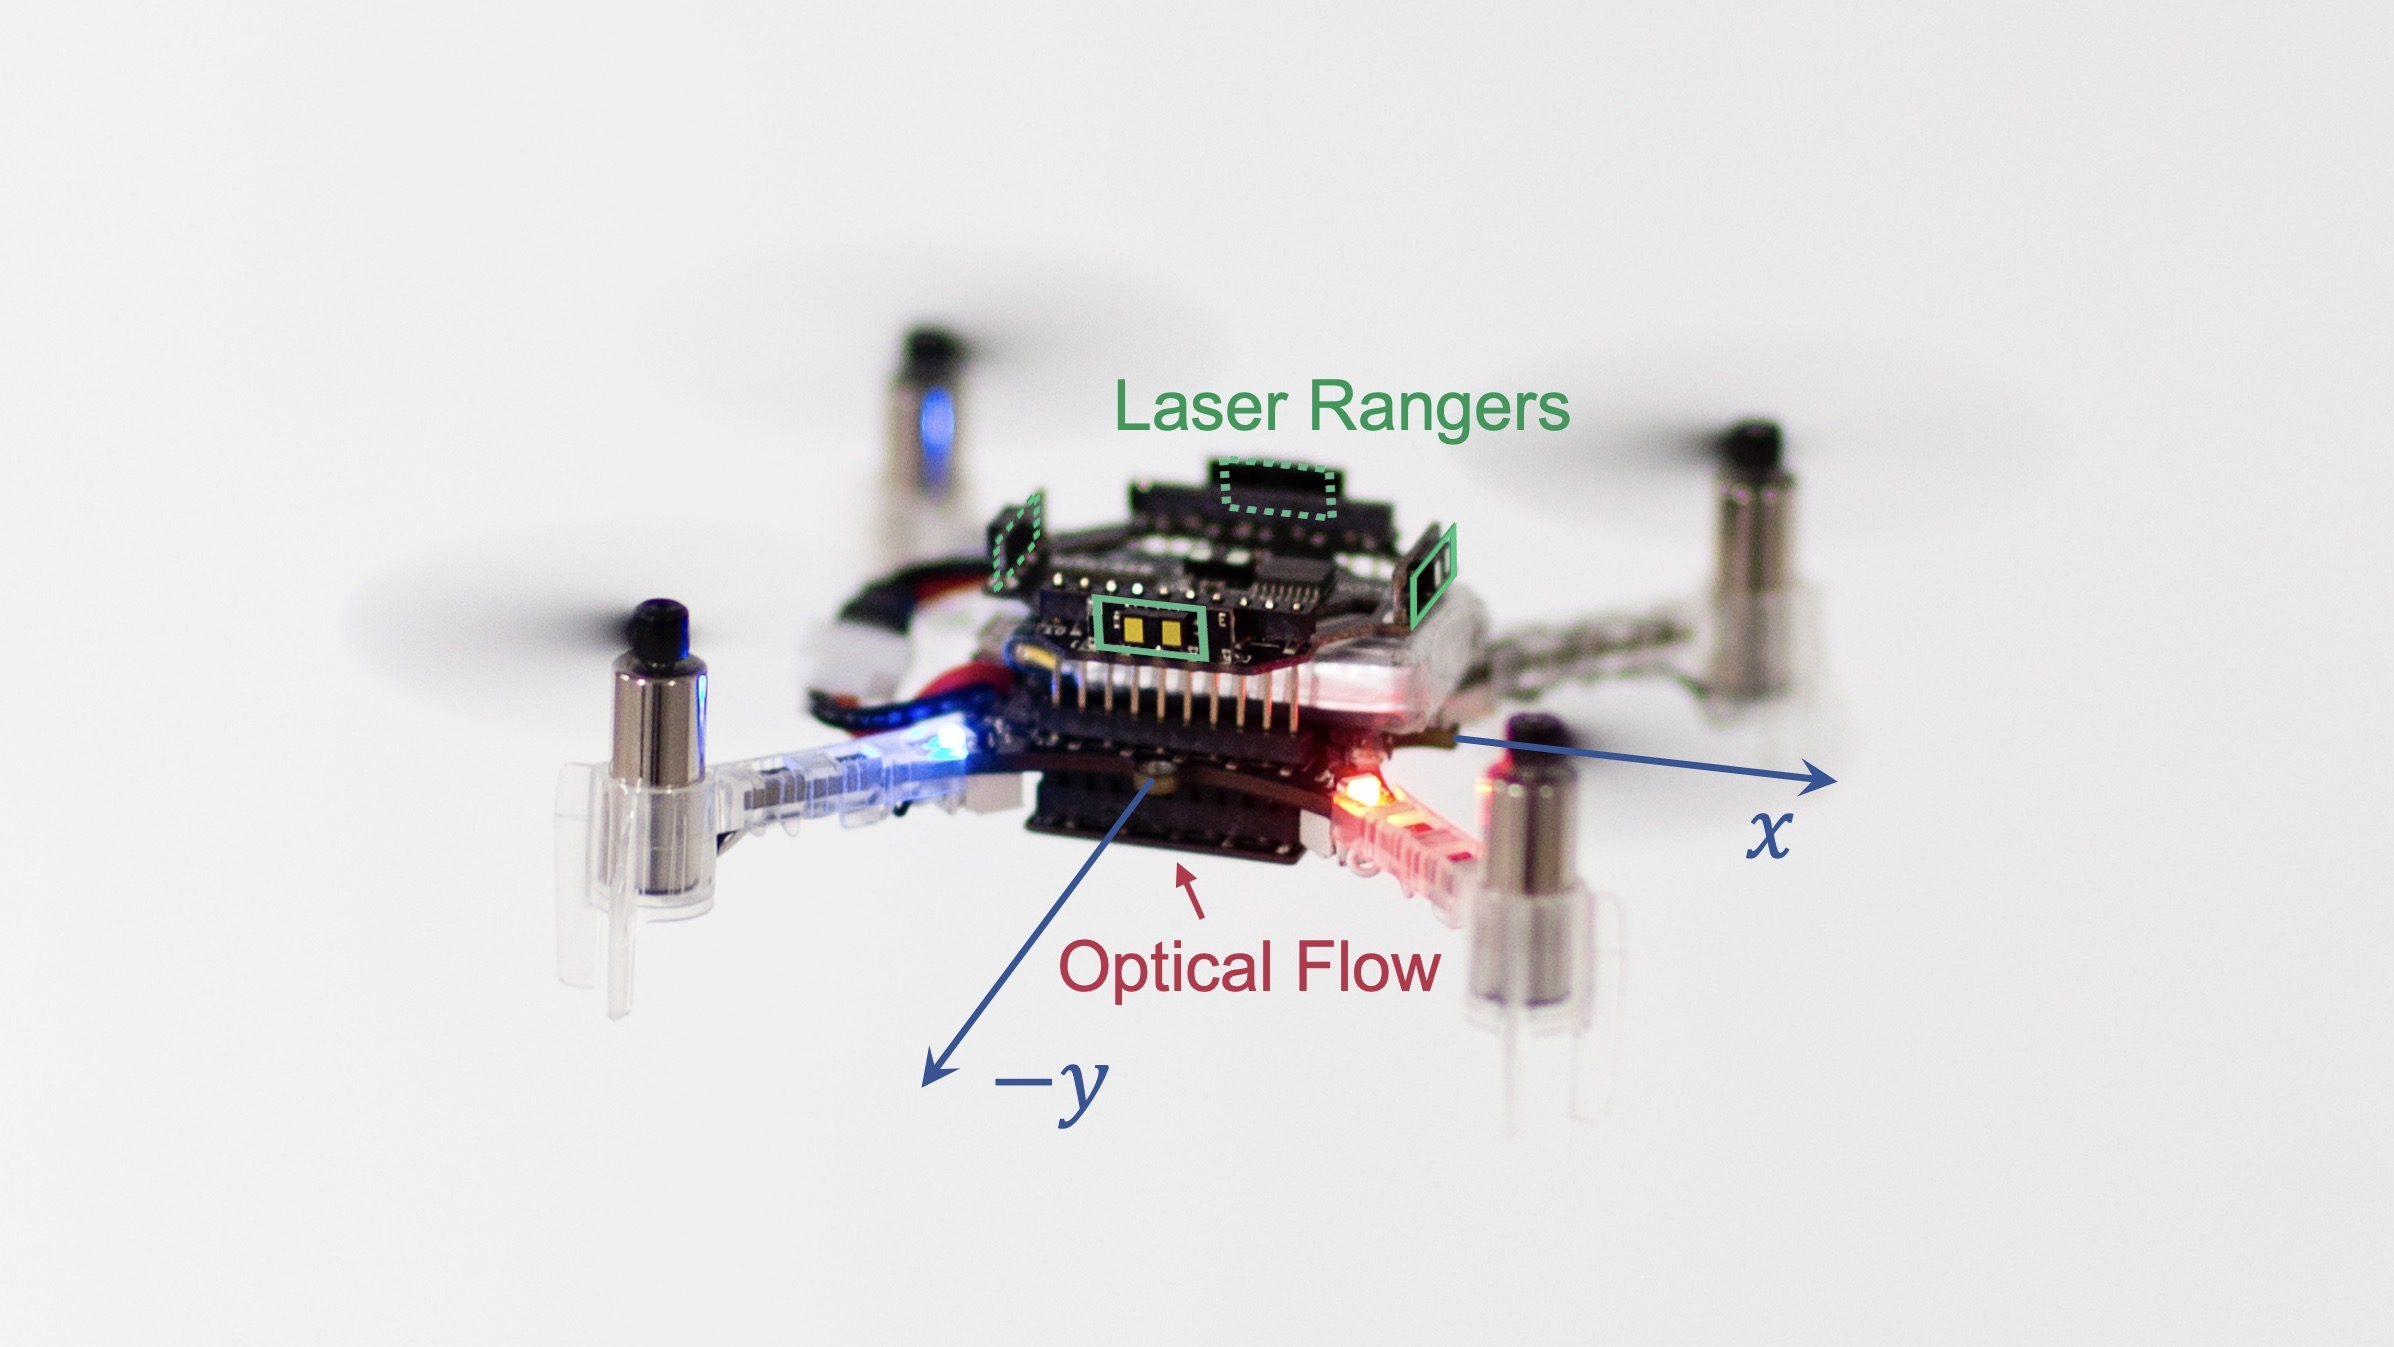
\includegraphics[width=.6\linewidth]{figures/content/chapter4/crazyflie.jpeg}
  \caption{带有4个激光器的微型无人机设备，用于探测障碍物}
  \label{fig:4_1}
\end{figure}

无人机的状态与观测部分中，本文选用Crazyflie 2.1 Brushless纳米四旋翼无人机作为实验平台。
如图\ref{fig:4_1}所示，该无人机在机体$x$轴和$y$轴的正负方向上分别安装了四个激光测距传感器，用于检测周围障碍物。
同时，无人机还配备了光流相机扩展版，用于估计飞行速度，从而实现底层飞行控制。
在导航任务中，系统状态空间$S$包含无人机自身状态、目标位置以及环境障碍物信息。
状态可以表示为
$s_{t}=\left\langle p, d_{g}, d_{o}\right\rangle$。
其中， $p$  表示无人机的全局位置；
$d_{g}=\left\|p-p_{g}\right\|_{2}$  表示无人机与目标点之间的欧氏距离；
$d_{o}$  为一个向量，用于表示无人机到周围障碍物的距离信息。
由于机载传感器数量和测量能力有限，无人机无法完全观测到完整的系统状态。
因此，在实际决策过程中，无人机仅能够获得部分观测信息。观测向量表示为
$o_{t}=\left\langle p, d_{g}, d_{l}\right\rangle$。
其中，$d_{l}$表示激光测距传感器的反射距离。
激光传感器的最大探测距离为4 m。
在真实飞行实验中，无人机的全局位置$p$以及目标距离$d_{g}$由外部运动捕捉系统提供。

为了适配所提出的算法，本文将动作空间$A$设计为离散化的速度控制指令，包括不同大小和方向的速度组合。
速度幅值被离散为$m$个指数间隔分布在区间$\left(0, v_{m}\right]$内的取值，其中$v_{m}$表示无人机允许的最大飞行速度。
由于激光传感器只能检测与激光束方向相交的障碍物，因此无人机的运动方向被离散为在区间 $[0,2 \pi)$内均匀分布的4个方向。

奖励函数通过人工设计，用于鼓励无人机尽快到达目标点，同时对发生碰撞或接近障碍物的行为进行惩罚。奖励函数定义为
\begin{equation}
  R\left(s_{t}, a_{t}\right)=\left\{\begin{array}{ll}
50, & d_{g}<d_{f} \\
5\left(d_{o}-d_{s}\right), & r_{d}<d_{o}<d_{s} \\
-25, & d_{o}<r_{d} \\
-0.1, & \text { otherwise }
\end{array}\right.
\end{equation}
其中，$d_{f}$表示到达目标点的判定阈值；$d_{o}$表示无人机到最近障碍物的距离；$d_{s}$表示安全距离阈值；$r_{d}$表示无人机机体半径。
通过上述奖励设计，可以引导无人机在保持安全距离的前提下快速到达目标位置，从而实现安全高效的自主导航。
\subsection{自适应风险倾向隐式分位数网络} 

为了能够在决策过程中动态调整策略的风险倾向，本文提出一种自适应风险倾向隐式分位网络（Adaptive Risk-Tendency Implicit Quantile Network，ART-IQN）算法。
该方法在分布式强化学习框架下构建，图\ref{fig:4_2}给出了 ART-IQN 的整体结构，其核心组成部分包括：
1）风险敏感隐式分位网络；
2）内在不确定性估计机制；
3）基于指数加权平均预测的不确定性预测方法，下文将分别对他们进行详细的阐述与说明。

\begin{figure}[htbp]
  \centering
  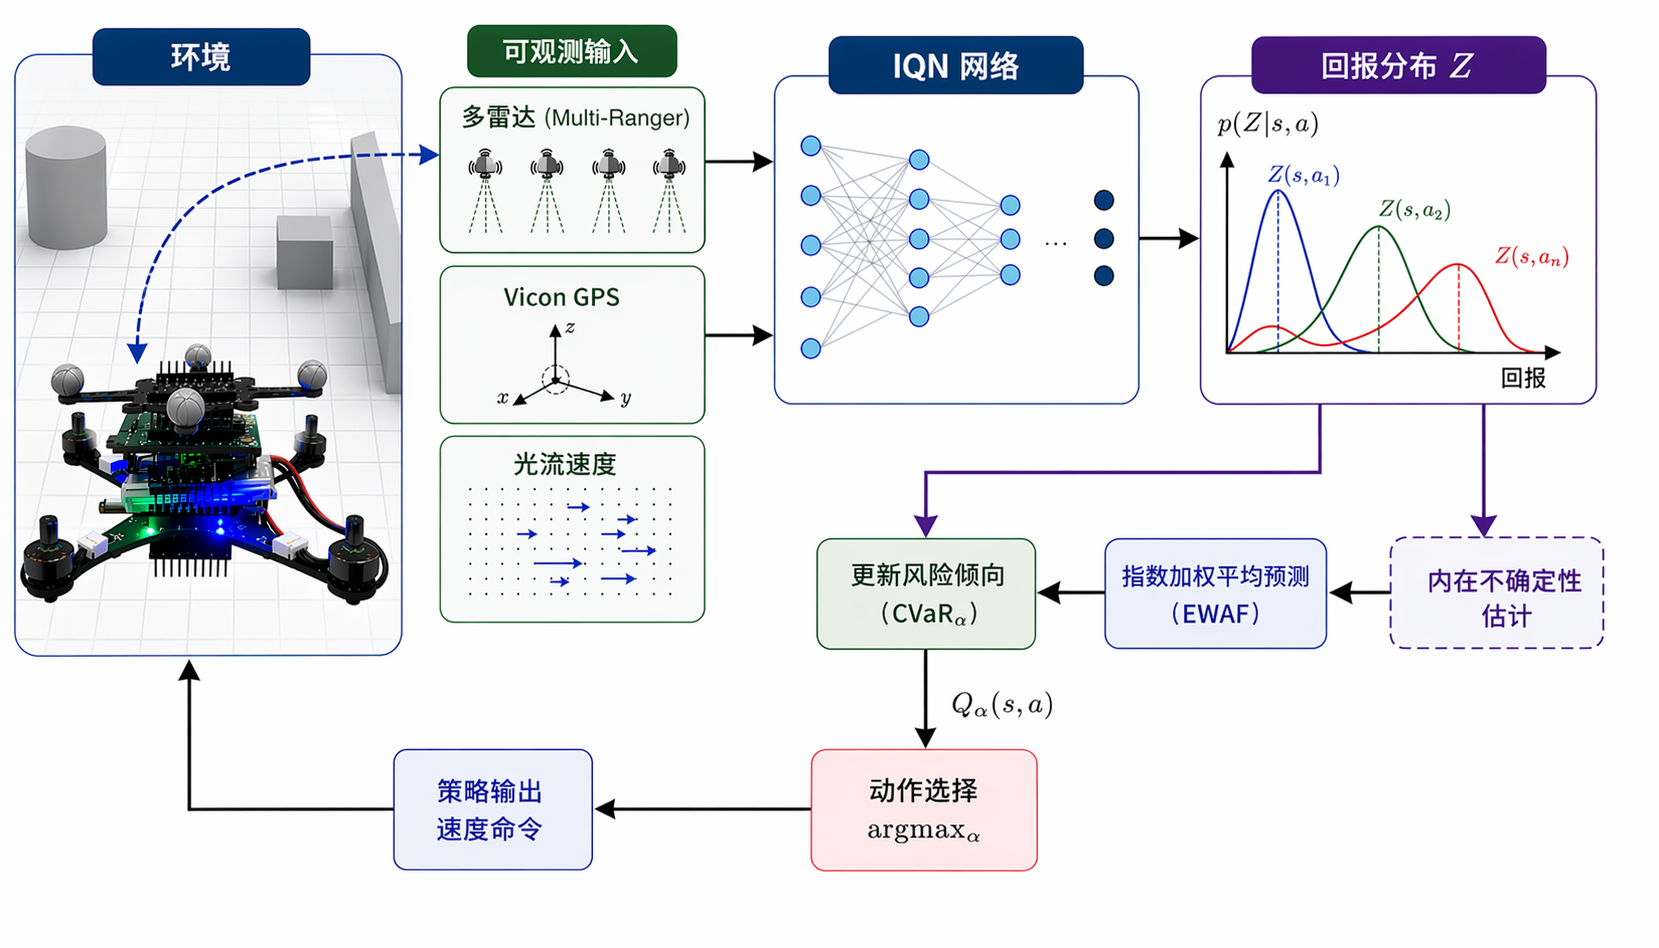
\includegraphics[width=.8\linewidth]{figures/content/chapter4/IQN.png}
  \caption{自适应风险倾向隐式分位网络框架}
  \label{fig:4_2}
\end{figure}

在分布式强化学习中，贝尔曼方程可以表示为
\begin{equation}
Z^{\pi}(s, a) \stackrel{D}{=} R(s, a)+\gamma Z^{\pi}\left(s^{\prime}, a^{\prime}\right)
\end{equation}
其中，符号$\stackrel{D}{=}$表示两个随机变量在分布意义下相等。
状态$s^{\prime}$和动作$a^{\prime}$的分布满足$s^{\prime} \sim P(s, a), a^{\prime} \sim \pi\left(\cdot \mid s^{\prime}\right)$。


在隐式分位数网络\cite{mokhtari2018iqn}方法中，我们使回报分布$Z^{\pi}(s, a$)通过其分位函数进行隐式表示，这种表示方式便于与不同风险度量方法结合，从而实现策略风险倾向的动态调整。
具体而言，分位函数由参数为$\theta$的神经网络进行近似表示：$Z_{\theta}^{\pi}(s, a ; \tau)$，
其中，$\tau \in[0,1]$表示分位水平。
为了训练该网络并优化参数$\theta$，需要进行分位回归\cite{buchinsky1998recent}，并采用Quantile Huber损失作为Wasserstein\cite{mokhtari2018iqn}距离的近似优化目标。

对于样本$\left(s, a, r, s^{\prime}\right)$，本文使用参数为$\theta^{\prime}$的神经网络对目标回报分布进行近似表示，并通过时间差分（Temporal Difference，TD）更新计算其误差。
其时序差分误差可表示为
\begin{equation}
\delta_{\tau, \tau^{\prime}}=r+\gamma Z_{\theta}^{\pi}\left(s^{\prime}, a^{\prime} ; \tau^{\prime}\right)-Z_{\theta}^{\pi}(s, a ; \tau)
\end{equation}
其中，$\tau$与$\tau^{\prime}$独立地从均匀分布中采样，即$\tau, \tau^{\prime} \sim U[0,1]$。

对应的$\tau$－分位Huber损失定义为
\begin{equation}
\begin{array}{l}
\rho_{\kappa}(\delta ; \tau)=|\tau-\mathbb{I}\{\delta<0\}| \frac{\mathcal{L}_{\kappa}(\delta)}{\kappa}, \text { with } \\
\mathcal{L}_{\kappa}(\delta)=\left\{\begin{array}{ll}
\frac{1}{2} \delta^{2} & \text { if }|\delta| \leq \kappa \\
\kappa\left(|\delta|-\frac{1}{2} \kappa\right) & \text { otherwise }
\end{array}\right.
\end{array}
\label{equ:Huber}
\end{equation}
其中, $\mathbb{I}$为指示函数，参数$\kappa$用于实现平滑梯度裁剪。
在实际训练中，通过采样$N$个分位值$\tau$以及$N^{\prime}$个目标分位值$\tau^{\prime}$，最终得到网络参数$\theta$的优化目标：
\begin{equation}
\mathcal{L}(\theta)=\frac{1}{N \cdot N^{\prime}} \sum_{i=1}^{N} \sum_{j=1}^{N^{\prime}} \rho_{\kappa}\left(\delta_{\tau_{i}, \tau_{j}^{\prime}} ; \tau_{i}\right)
\label{equ:lossfunction}
\end{equation}
通过对该损失函数进行反向传播优化，可以最小化当前回报分布$Z^{\pi}(s, a)$与目标分布$R(s, a)+\gamma Z^{\pi}\left(s^{\prime}, a^{\prime}\right)$之间的Wasserstein距离。

在风险敏感策略与风险度量方面，分布式强化学习通过对回报分布进行建模，使策略能够结合不同的风险度量指标进行决策。
通常情况下，可以通过扭曲期望来构造风险敏感策略。
该期望是在回报分布上施加一个单调非减的扭曲函数$\beta:[0,1] \rightarrow[0,1]$，并满足$\beta(0)=0, \beta(1)=1$。
在该扭曲函数作用下，回报分布的扭曲期望定义为$Q_{\beta}=\int_{0}^{1} F_{Z}^{-1}(\tau) d \beta(\tau)$。
其中，$F_{Z}^{-1}(\tau)$表示回报分布的分位函数。
实际上，该期望可以通过对分位值进行加权求和来近似计算。
具体而言，通过从均匀分布中采样$K$个分位值$\tilde{\tau}\sim U[0,1]$来近似$Q_{\beta}$，可得到基于样本的风险敏感策略：
\begin{equation}
\pi_{\beta}(s)=\arg \max _{a \in A} \frac{1}{K} \sum_{k=1}^{K} Z_{\beta}\left(\tilde{\tau}_{k}, s, a\right)
\end{equation}

通过改变分位值$\tau$的采样方式，可以生成不同风险偏好的策略。
本文采用条件风险价值（Conditional Value-at-Risk，CVaR）\cite{filippi2020conditional}作为扭曲函数。
CVaR是一种满足一致性性质的风险度量指标\cite{majumdar2019should}，在生成不同风险偏好水平方面具有良好的灵活性与实用性。
在隐式分位数网络框架下，可通过将分位采样范围从$\tau \sim U[0,1]$调整为$\tau \sim U[0, \alpha]$来实现 CVaR 计算，其中, $\alpha$表示风险水平参数。
当$\alpha$ 趋近于0时，策略将更加保守；当$\alpha=1$时，策略退化为风险中性策略。

在强化学习任务中，风险的重要来源之一是内在不确定性，该不确定性主要来源于环境的随机性以及系统的部分可观测性。
与认知不确定性\cite{clements2019estimating}不同，内在不确定性并不会随着经验积累而消失。
在分布式强化学习中，回报分布的离散程度能够反映环境的不确定性水平\cite{moskovitz2021deep}。
文献\citen{mavrin2019distributional}通过利用回报分布上尾条件方差的衰减特性来提升探索效率。
受到该方法的启发，本文选择回报分布的下尾条件方差来刻画内在不确定性，并据此实现策略风险倾向的动态调整。
值得注意的是，下尾一半区间的条件方差可等价表示为右截断方差（Right Truncated Variance，RTV）：
\begin{equation}
R T V=\frac{2}{N} \sum_{i=1}^{N / 2}\left(F_{Z}^{-1}\left(\tau_{i}\right)-F_{Z}^{-1}\left(\tau_{N / 2}\right)\right)^{2}
\end{equation}
其中,$\tau_{i}$  表示第$i/N$个分位水平。
直观上看，RTV 对负收益区域更加敏感，因此能够有效刻画潜在风险。
本文在计算RTV时采用分布的中位数作为参考点，而不是均值，以提升统计稳定性\cite{maronna2019robust}。
需要注意的是，在本文方法中，分位函数$F_{Z}^{-1}(\tau)$通过神经网络输出的分位估计$Z_{\theta}^{\pi}(s, a ; \tau)$进行近似计算。

最后我们介绍基于指数加权平均预测的风险倾向自适应方法。
在本文提出的框架中，策路的风险倾向通过CVaR的取值进行调节。
为了将 CVaR 表示为 RTV 的函数关系，本文利用指数加权的类别分布对 CVaR 进行建模。

具体而言，考虑一个包含两个logits的类别分布$C$：$C_{i}=\frac{\exp \left(w_{i}\right)}{\sum_{i} \exp \left(w_{i}\right)}, \quad i=1,2$。
其中，$w_{i} \in \mathbb{R}$。
通过令$\alpha=C_{1}$,即可将 CVaR 的取值限制在区间$(0,1)$内，并通过调整logits权重实现风险水平的调节。
具体的，在每个时间步$t$, CVaR参数通过以下方式进行更新：利用步长$\eta$ 和反馈信号$f$对权重$w_{i}$进行调整：
\begin{equation}
w_{1}=w_{1}-\eta f, \quad w_{2}=w_{2}+\eta f
\end{equation}
其中反馈信号定义为$f=R T V_{t}-R T V_{t-1}$
该反馈量反映了内在不确定性的变化程度。
为避免 CVaR 的取值过小甚至趋近于0，在类别分布中额外引入一项$\sum_{i} \exp \left(w_{i}\right) / b$。
该项同时加入到$C_{i}(i=1,2)$的分母以及$C_{1}$的分子中，从而将 CVaR 的取值范围限制在$\left(\frac{1}{b+1}, 1\right)$。
例如，当$b=9$时，得到$\alpha \in(0.1,1)$。

能够根据内在不确定性变化自适应调整风险倾向的整体ART-IQN算法流程如算法\ref{alg:artiqn}所示。
从原理上看，当 RTV 持续增大且当前 CVaR 值较高时，无人机会通过减小 CVaR 的取值来表现出更加保守的决策行为，从而降低潜在风险。


\begin{algorithm}[H]
  \caption{自适应风险倾向隐式分位网络无人机导航算法}
  \label{alg:artiqn}
  \begin{algorithmic}[1]
  
  \State \textbf{输入：} 训练完成的 $IQN_{\theta}$；动作集合 $A$，参数 $K, N, w_1, w_2, b, \eta$
  \State 初始化状态 $s$，CVaR 参数 $\alpha$
  
  \While{$d_g > d_f$ 且 $t \le H$}
  
  \State 从状态 $s_t$ 得到观测 $o_t \gets \langle \mathbf{p}, d_g, d_l \rangle$
  
  \State 获取分位函数 $Z_{\theta}(o_t,a;\tau)=IQN_{\theta}(o_t;\tau)$
  
  \State 进行失真采样 $\tilde{\tau}_k \sim \mathcal{U}[0,\alpha],\; k=1,\dots,K$
  
  \State $a_t \gets 
  \displaystyle \arg\max_{a\in A}
  \frac{1}{K}\sum_{k=1}^{K} Z_{\theta}(o_t,a;\tilde{\tau}_k)$
  
  \State 计算右截断方差 $RTV_t \gets 
  \displaystyle \frac{2}{N}
  \sum_{i=1}^{N/2}
  \left(
  Z_{\theta}(o_t,a_t;\tau_i)
  -
  Z_{\theta}(o_t,a_t;\tau_{N/2})
  \right)^2$
  
  \State $f_t \gets RTV_t - RTV_{t-1}$
  
  \State $w_1 \gets w_1 - \eta f_t$
  
  \State $w_2 \gets w_2 + \eta f_t$
  
  \State $\alpha \gets 
  \displaystyle
  \frac{(b+1)\exp(w_1)+\exp(w_2)}
  {(b+1)\sum_i \exp(w_i)},\; i=1,2$
  
  \EndWhile
  
  \end{algorithmic}
  \end{algorithm}

\subsection{网络模型结构设计与实现方法}
在前文对所提出算法的基本原理与核心思想进行介绍的基础上，本节进一步给出强化学习智能体Agent与IQN模型的具体实现过程。
在网络模型中，智能体是整个算法的核心组成部分，其主要功能是与环境进行交互并学习，以实现特定的任务目标。
本小节将详细介绍智能体的设计与实现，包括其结构、动作空间、学习算法等方面。
智能体采用了深度强化学习中的双深度Q网络（Double Deep Q-Network，DDQN）的变体——基于分位数回归的IQN网络。
这种网络结构结合了分位数回归的思想，能够更好地处理不确定性，为智能体提供更准确的价值估计。
\subsubsection{双网络结构}
智能体采用的双网络结构，包括本地网络和目标网络。
这种结构常用于深度强化学习算法中，如深度强化学习网络及其变体，用以减少训练过程中目标值剧烈波动带来的不稳定性。
本地网络负责根据当前状态实时计算动作价值的分位数估计，指导智能体进行动作选择。
而目标网络则用于生成训练过程中的目标值，其参数不参与实时更新，而是通过软更新方式定期从本地网络复制，从而为目标值提供更稳定的估计。
两个网络的结构完全相同，均由IQN类定义。
IQN模型以状态为输入，输出对应动作价值的分位数信息，能够有效刻画价值分布，提升策略在不确定性环境下的表现。
其核心参数包括状态维度、动作维度、网络层大小、步长、随机种子、分布扭曲因子、风险价值卷积以及方差采样数。
\subsubsection{构建智能体的动作空间}
在离散动作空间中，智能体的决策本质上是在有限个候选动作中选择最优执行策略。
为覆盖多种运动方向与速度组合，本文设计了构建智能体的动作空间的方法。
具体而言，动作空间由方向与速度两个维度组合生成。
方向维度通过将圆周$[0,2 \pi)$等分为$N_{direction}$个离散方向实现；
速度维度则采用非线性映射生成$N_{speed}$个离散速度值来生成一系列可能的动作。
速度生成公式如下：
\begin{equation}
v_{i}=\frac{e^{(i+1) / N_{speed}}-1}{e-1} \cdot v_{\max }, \quad i=0,1, \ldots, N-1
\end{equation}
其中 ,$v_{max }$为无人机最大速度。
该公式利用指数函数的特性，使得速度值在低速区间分布更密集，高速区间分布更稀疏，符合实际运动中低速调整更频繁的需求。

随后，通过对所有方向与速度进行笛卡尔积，得到动作候选集合。
每个动作由一个二维向量ActionXY表示，其分量为智能体在水平面上的速度分量，计算方式如下：
\begin{equation}
\text { Action }=(v \cdot \cos (\theta), v \cdot \sin (\theta))
\end{equation}
其中，$\theta$为离散方向角， $v$为离散速度值。
最终生成的动作空间大小为 $N_{direction}  \times  N_{speed}$，该方法保证了动作空间对运动方向的均匀覆盖和对速度的合理分布，兼顾了控制的精细度与计算效率。
\subsubsection{模型训练算法}
在模型训练阶段，智能体通过与环境交互不断收集状态转移数据，并利用经验回放机制对历史交互数据进行存储。
经验回放缓冲区（Replay Buffer）中每条数据通常表示为一个五元组：$\left(s_{t}, a_{t}, r_{t}, s_{t+1}, d_{t}\right)$
其中，$s_{t}$表示当前时刻的状态，$a_{t}$表示执行的动作，$r_{t}$表示获得的即时奖励，$s_{t+1}$表示下一时刻的状态，$d_{t}$为终止标志，用于指示当前状态是否为终止状态。

在每一次训练迭代过程中，首先从经验回放缓冲区中随机采样一个批量（batch）的经验数据，从而打破样本之间的时间相关性，提高训练稳定性。
随后利用目标网络计算下一状态的分布式Q值。
对于每个样本，通过选择具有最大Q值的动作来构建目标值，其计算形式为
\begin{equation}
Q_{\text {target }}=r_{t}+\gamma^{n}\left(1-d_{t}\right) \max _{a} Q_{\text {target }}\left(s_{t+1}, a\right)
\end{equation}
其中, $\gamma$ 为折扣因子，用于衡量未来奖励的重要程度, $n$为多步回报步数,$d_{t}$  为终止标志，当到达终止状态时未来回报不再累。

通过上述公式可以得到每个样本对应的目标 Q 值。
随后利用本地网络计算当前状态$s_{t}$在执行动作$a_{t}$时的预测Q值。
由于本文采用的是分布式强化学习方法，网络输出的是一组分位数Q 值，因此可以表示为：
\begin{equation}
Q_{\text {expected }}=Z_{\theta}\left(s_{t}, a_{t}\right)
\end{equation}
其中,$Z_{\theta}$表示参数为$\theta$的分位数价值函数。

紧接着为了度量预测值与目标值之间的差异，首先计算时序差分误差（Temporal Difference Error）：
\begin{equation}
\delta_{i j}=Q_{\text {target }}^{(j)}-Q_{\text {expected }}^{(i)}
\end{equation}
其中，$i$表示当前网络输出的第$i$个分位数,$j$表示目标分布中的第$j$个分位数。

由于强化学习训练过程中误差可能较大，为了提高训练稳定性并减小异常值对训练的影响，本文采用上小节定义的Huber 损失函数对 TD 误差进行计算。
根据上小节中算法的原理最终计算得到损失函数之后,通过反向传播（Backpropagation）对网络参数进行更新，并采用梯度下降算法优化模型参数。
最后，为了保证训练过程的稳定性，采用软更新策略逐步更新目标网络参数，其更新公式为
\begin{equation}
\theta_{\text {target }} \leftarrow \tau \theta_{\text {local }}+(1-\tau) \theta_{\text {target }}
\end{equation}
其中,$\tau$为软更新系数，一般取较小值（如 0.001 ）。
通过该方式可以使目标网络缓慢跟随本地网络更新，从而减少训练震荡，提高算法的收敛稳定性。
模型训练迭代的流程如算法\ref{alg:trainingalg}所示
\begin{algorithm}[htbp]
  \caption{IQN网络模型训练流程}
  \label{alg:trainingalg}
  \begin{algorithmic}[1]
  
  \Require 经验回放缓冲区 $D$，批量大小 $N$，折扣因子 $\gamma$，软更新系数 $\tau$
  
  \For{每一次训练迭代}
  
  \State 从经验回放缓冲区 $D$ 中随机采样一批经验数据 $(s_t,a_t,r_t,s_{t+1},d_t)$
  
  \State 计算目标 Q 值：$Q_{target}=r_t+\gamma^n(1-d_t)\max_a Q_{target}(s_{t+1},a)$
  
  \State 使用本地网络计算当前状态动作对应的分位数 Q 值： $Q_{expected}=Z_{\theta}(s_t,a_t)$
  
  \State 计算时序差分误差：$\delta_{ij}=Q_{target}^{(j)}-Q_{expected}^{(i)}$
  
  \State 基于公式\ref{equ:Huber}计算 Huber 损失
  
  \State 基于公式\ref{equ:lossfunction}计算总体损失函数
  
  \State 通过反向传播更新本地网络参数
  
  \State 对目标网络进行软更新：$\theta_{target}\leftarrow\tau\theta_{local}+(1-\tau)\theta_{target}$

  
  \EndFor
  
  \end{algorithmic}
  \end{algorithm}

\subsubsection{动作选择策略}
在强化学习过程中，智能体需要在探索与利用之间取得平衡。探索是指尝试新的动作以获取更多环境信息，而利用则是选择当前估计最优的动作以获得更高的累计回报。
为了实现二者之间的有效权衡，本文采用$\varepsilon$－贪心策略进行动作选择。

在训练初期，为了充分探索环境，智能体以较大的概率  $\varepsilon$  随机选择动作；
随着训练的进行， $\varepsilon$  逐渐减小，从而使智能体以更高概率选择当前估计最优的动作，以提高策略的稳定性和收玫速度。

具体而言，在每个决策时刻，首先将当前环境状态$s_{t}$输入到训练好的IQN网络中，得到各个动作对应的价值函数估计：
\begin{equation}
Q\left(s_{t}, a\right)=Z_{\theta}\left(s_{t}, a\right)
\end{equation}
随后根据$\varepsilon$－贪心策略进行动作选择，其概率规则可以表示为：
\begin{equation}
a_{t}=\left\{\begin{array}{ll}
\arg \max _{a} Q\left(s_{t}, a\right), & \text { with probability } 1-\varepsilon \\
\operatorname{random} \text { action, } & \text { with probability } \varepsilon
\end{array}\right.
\end{equation}
当随机数大于$\varepsilon$时，智能体选择当前 Q 值最大的动作。否则，从动作空间$A$中随机选择一个动作。

此外，为了保证环境交互的稳定性，在部分时间步中智能体会保持上一时刻的动作不变，从而减少频繁动作切换带来的系统不稳定问题。最终，智能体输出所选择的动作索引及其对应的实际控制动作，用于与环境进行交互。
\subsubsection{分位数网络IQN}
在网络实现中，隐式分位数网络被实现为一个继承自\texttt{torch.nn.Module}的深度神经网络结构，并在智能体中分别作为本地网络和目标网络使用。
该模型用于估计状态一动作对的回报分布，并通过分位数回归的方式对动作价值函数进行建模。与传统 DQN 直接输出 Q 值不同，IQN 网络输出的是不同分位数下的价值估计$Z_{\theta}(s, a, \tau)$，从而能够更细致地刻画回报的不确定性。

在网络结构上，IQN 主要由输入层、分位数嵌入层、隐藏层以及输出层组成。
首先，输入状态$s$经过线性层进行特征映射，并通过ReLU 激活函数得到状态特征表示：
\begin{equation}
h=\operatorname{ReLU}\left(W_{s} s+b_{s}\right)
\end{equation}
其中，$W_{s}$和$b_{s}$分别为权重和偏置参数。
在分位数建模部分，模型首先从均匀分布中随机采样分位数参数：$\tau \sim U(0,1)$。
随后利用余弦函数对分位数进行嵌入表示：
$\phi(\tau)=\cos (\pi i \tau), \quad i=1,2, \ldots, n_{\cos }$。
其中，$n_{c o s}$表示余弦嵌入维度。
在代码实现中，通过上述方法完成分位数采样及余弦嵌入计算。
若采用风险敏感策略，则对采样得到的分位数进行缩放处理，以调整模型对回报分布不同区间的关注程度。
随后，将得到的分位数嵌入特征通过线性映射转换为与状态特征相同的维度，并与状态特征进行逐元素乘法融合：
$f(s, \tau)=h(s) \odot \phi(\tau)$。
融合后的特征被输入到多层全连接隐藏层中，通过非线性变换进一步提取高层语义特征。最后，通过输出层得到每个动作在不同分位数下的价值估计
$Z_{\theta}(s, a, \tau)$

\subsection{模型训练与模拟实验结果分析}
本文中设计了一个类似OpenAI Gym\citen{brockman2016openai}的二维环境进行本实验的模型训练与仿真实验，其中状态、观测和动作空间的定义如上文\ref{sec:stateDefine}节所述。
为实现快速仿真，将无人机建模为质点，并假设速度指令能立即执行。
在仿真时间中，状态每$T$秒更新一次。
我们利用域随机化技术\citen{tobin2017domain}来训练可泛化到不同场景的策略。
具体来说，每个训练阶段中，目标距离在$d_{g} \sim U[5,7](m)$范围内均匀采样，智能体在固定起始点初始化。
每一个情节中，障碍物的数量、形状和位置都是随机生成的，如图\ref{fig:4_3}所示。
为简化计算，智能体测距激光和障碍物轮廓被建模为线段。
在每个测距激光的测量值中添加均值$\mu=0.0$、标准差$\sigma=0.01$的高斯噪声$N(\mu, \sigma)$，以模拟传感器噪声。

在上述环境设定下，采用渐进式训练策略以提升模型鲁棒性，具体流程为采用循序渐进的方式训练无人机，即随着训练过程推进，环境复杂度逐渐增加。
训练的第一阶段，随机生成的障碍物数量相对较少，$n_{o b s} \in[0,5]$。
在训练多轮阶段（直至导航成功率达到 0.8 ）后，通过增加障碍物数量来提高环境复杂度，$n_{o b s} \in[6,12]$。
为确保无人机在各种风险倾向下积累丰富的经验，每一个训练阶段中CVaR值在$\alpha \sim U(0,1]$范围内均匀采样。
如果发生碰撞或在$H$个时间步内未到达目标，该训练阶段即终止。
当平均回报在经验上趋于收玫时，整个训练过程结束。
在 Nvidia RTX 3070Ti 核心 GPU 上，训练耗时约半小时。

\begin{figure}[htbp]
  \centering
  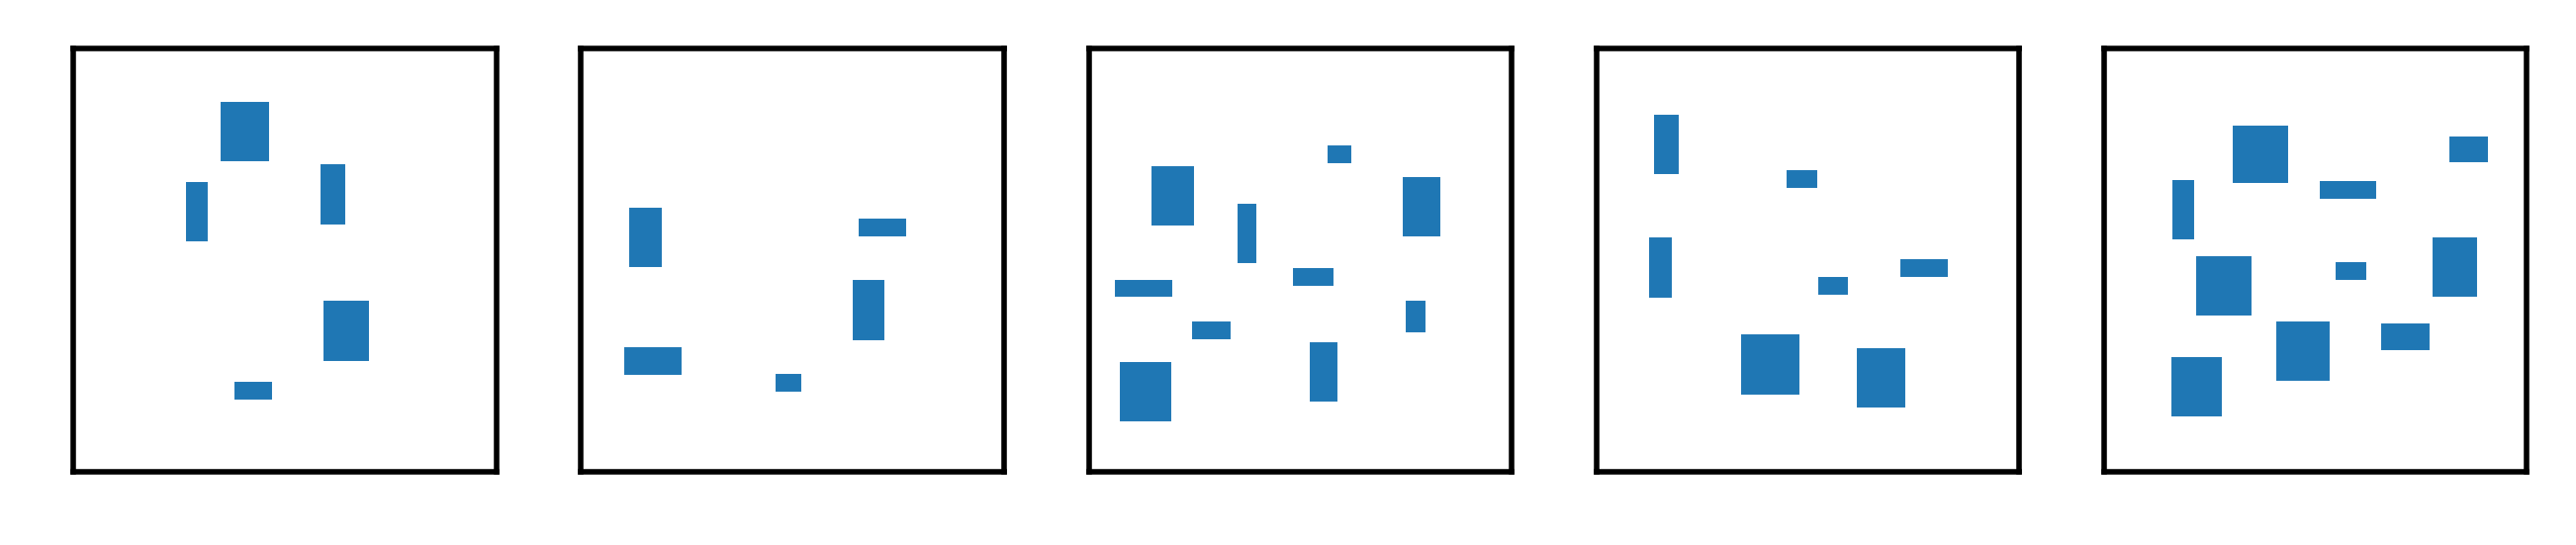
\includegraphics[width=.8\linewidth]{figures/content/chapter4/obstacles.png}
  \caption{随机生成的仿真训练环境}
  \label{fig:4_3}
\end{figure}
在训练过程中，智能体被建模为一个全连接网络，有 3 个隐藏层，每层 512 个单元。
除输出层外，每个全连接层后都接有 ReLU\citen{fred2018deep}激活函数。
我们使用Adam\citen{reyad2023modified}优化器，学习率为 lr。
每D个训练阶段进行一次更新，从大小为E的经验回放缓冲区中抽取批量大小为B的样本。
使用的超参数与值列于表\ref{tab:hyperparams}。

\begin{table}[htbp]
  \centering
  \begin{tabular}{ll|ll|ll|ll}
    \hline
    $lr$ & $2 \times 10^{-4}$ & $v_m$ & $1\ [m/s]$ & $D$ & $5$ & $N, N'$ & $16$ \\
    $E$ & $5 \times 10^{4}$ & $r_d$ & $0.05\ [m]$ & $K$ & $64$ & $m$ & $3$ \\
    $\gamma$ & $0.99$ & $d_f$ & $0.1\ [m]$ & $B$ & $32$ & $b$ & $9$ \\
    $T$ & $0.1\ [s]$ & $d_s$ & $0.2\ [m]$ & $H$ & $200$ & $\eta$ & $0.5$ \\
    \hline
  \end{tabular}
  \caption{超参数的符号与值}
  \label{tab:hyperparams}
\end{table}

在无人机导航仿真评估中，为了展示我们算法的有效性，我们将ART-IQN与具有多个风险倾向$\alpha=\{0.1,0.25,0.5,0.75,1.0\}$的IQN进行比较。
此外，我们还训练了一个DQN智能体作为对照，训练过程与所提出的算法相同。
我们比较了不同智能体在不同环境下的平均回合返回值、成功率、碰撞率和平均导航时间。
具体来说，评估在三组环境上进行，每组环境包含100个不同的随机环境，每个智能体的节点数分别为$n_{obs}=\{2,6,12\}$。

\begin{table}[htbp]
  \centering
  \caption{CVaR 性能指标对比}
  \label{tab:cvar_comparison}
  \begin{tabular}{|c|c|*{9}{c|}}
    \hline
    \multirow{2}{*}{方法} & \multirow{2}{*}{CVaR} & \multicolumn{3}{c|}{成功率} & \multicolumn{3}{c|}{碰撞率} & \multicolumn{3}{c|}{导航时间 [s]} \\
    \cline{3-11}
    & & n=26 & n=12 & n=6 & n=26 & n=12 & n=6 & n=26 & n=12 & n=6 \\
    \hline
    DQN  & - & 0.85 & 0.65 & 0.56 & 0.13 & 0.31 & 0.39 & 5.23 & 8.11 & 8.34 \\
    \hline
    \multirow{5}{*}{IQN} & 0.1 & 0.87 & 0.74 & 0.59 & 0.09 & 0.15 & 0.17 & 5.41 & 12.52 & 18.52 \\
    & 0.25 & 0.88 & 0.72 & 0.67 & 0.10 & 0.17 & 0.25 & 5.31 & 10.23 & 13.23 \\
    & 0.5 & 0.87 & 0.73 & 0.66 & 0.11 & 0.19 & 0.28 & 5.30 & 8.46 & 9.46 \\
    & 0.75 & 0.84 & 0.69 & 0.62 & 0.13 & 0.22 & 0.31 & 5.25 & 8.57 & 8.60 \\
    & 1.0 & 0.86 & 0.67 & 0.57 & 0.12 & 0.30 & 0.41 & 5.12 & 7.89 & 8.05 \\
    \hline
    ART-IQN & - & 0.87 & 0.77 & 0.70 & 0.11 & 0.17 & 0.15 & 5.32 & 8.26 & 11.76 \\
    \hline
  \end{tabular}
\end{table}

表\ref{tab:cvar_comparison}通过对比DQN、不同风险偏好下的 IQN 以及ART-IQN，展示了定量实验结果。
在所有测试环境中，DQN的表现与风险中性的IQN相近。
当障碍物数量$n_{obs}=2$时，环境相对简单，所有智能体均能以较高的成功率和较低的碰撞率完成导航任务。
当$n_{obs}=6$时，采用较低CVaR值的IQN智能体相比高CVaR值的智能体碰撞率更低，但其任务完成时间更长，超时率也更高。
相比之下，ART-IQN 在成功率达到0.77的同时，保持了较低的碰撞率，且平均导航时间仅比风险中性策略长出0.37秒。
在$n_{obs}=12$的情况下，所有智能体的平均回报和成功率均有所下降。
这一下降可归因于智能体所面临的严重部分可观测性问题。在低CVaR设置下超时情况更常见，而在高CVaR设置下碰撞更为频繁。
相比之下，ART-IQN 在成功率和碰撞率方面均表现最佳，同时导航时间也维持在合理范围内。

\begin{figure}[htbp]
  \centering
  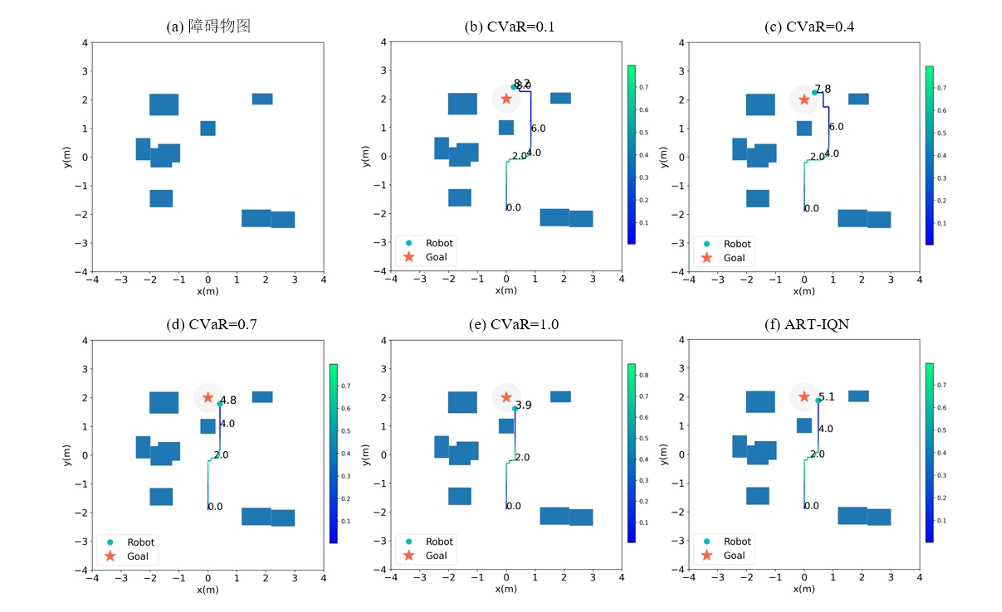
\includegraphics[width=.9\linewidth]{figures/content/chapter4/uvasimulation.png}
  \caption{不同风险倾向的无人机行为和导航时间比较}
  \label{fig:4_4}
\end{figure}

我们选取一次随机生成障碍物数量为9个的实验结果作为典型样例进行定行分析，如图\ref{fig:4_4}所示。
其中图\ref{fig:4_4}（a）是障碍物图，图\ref{fig:4_4}（b）-图\ref{fig:4_4}（e）是具有不同CVaR的IQN模型结果，图\ref{fig:4_4}（f）是ART-IQN模型结果，路线上的颜色表示飞行时的速度，数字表示飞行路线的长度。
当CVaR的数值为1时，无人机会以优先到达目的地为目标，而忽略了因接近障碍物导致的碰撞风险，所以在图\ref{fig:4_4}（e）中，无人机后半程以紧贴方形障碍物线路飞行，并以最短的3.9米总路程到达终点。
随着CVaR数值的下降，无人机会逐渐提高与障碍物碰撞的警觉性，这会在周围有障碍物的情况下，优先保障无人机与障碍物处于一定的安全距离，但牺牲了飞行的速度以及可能导致更远的飞行路线，甚至在CVaR数值为0.4和0.1的情况下，无人机在接近终点时收到终点左侧矩形障碍物影响，都出现不同程度进一步再向y轴正方向飞行的情况。

相比之下，在图\ref{fig:4_4}（f）中，ART-IQN模型的无人机通过动态调整CVaR，在避障效率与风险控制间取得平衡，其路径在周围障碍物变多时保持较低的速度以及一定的距离，当周围障碍物变少时，提高飞行的速度。
在飞行刚开始时，飞机速度偏小，这是因为刚开始还并不了解周围的环境，不确定性较高，随着飞机向前接近目标点方向飞行，周围障碍物稀松并且距离较远，速度开始加快，当发现坐标点大约为（0，1）的障碍物时，飞机进行避障处理且降低飞行速度，直至抵达飞行终点。


\begin{figure}[htbp]
  \centering
  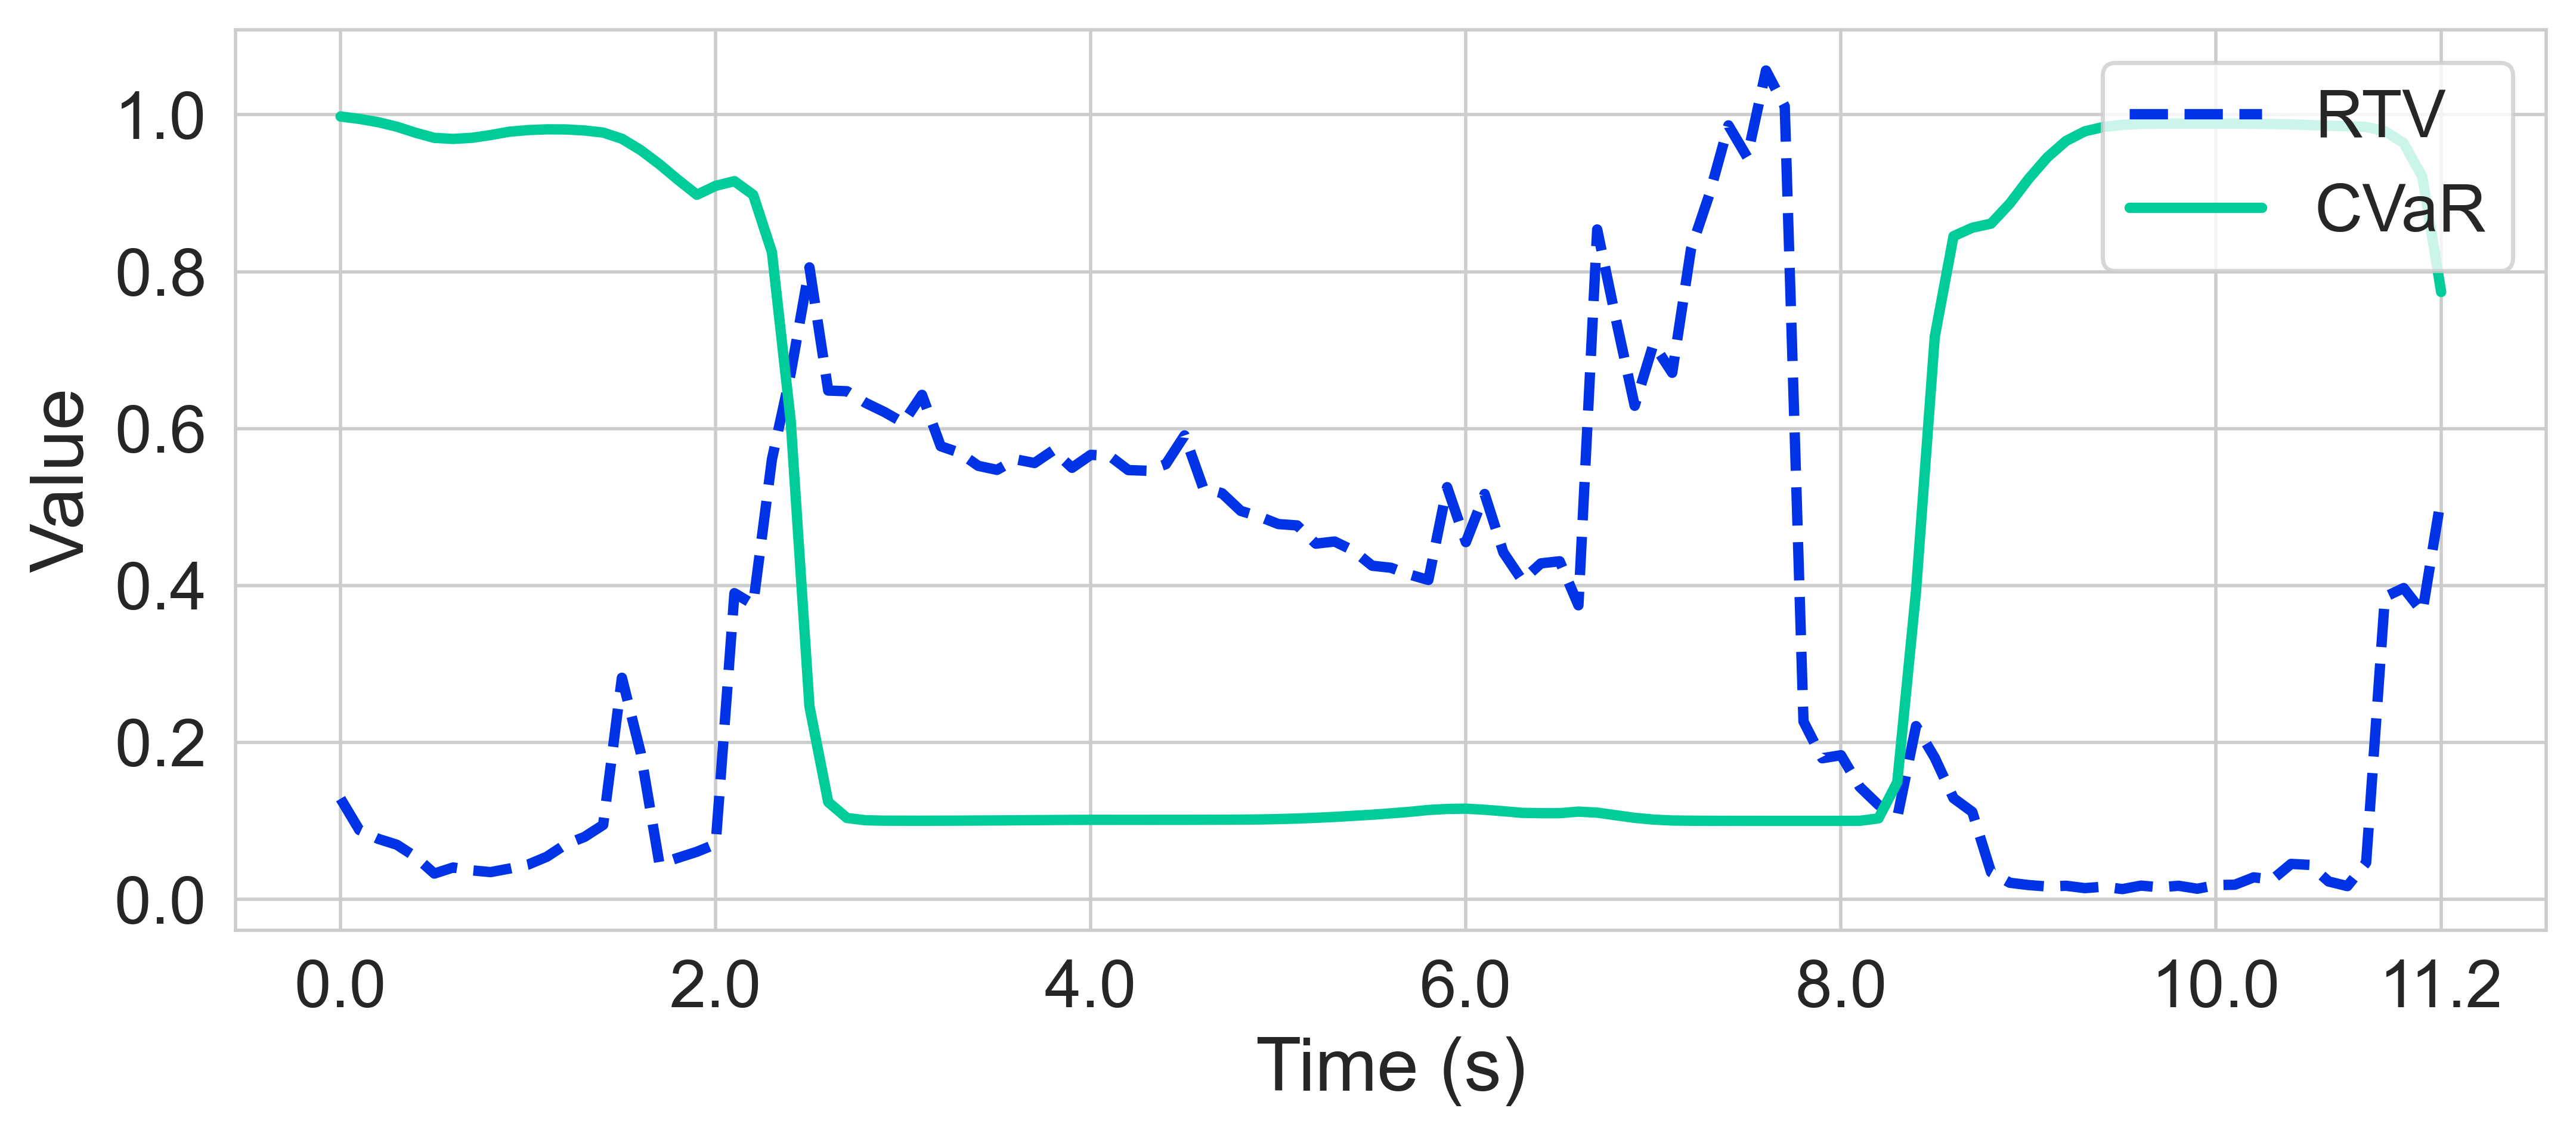
\includegraphics[width=.8\linewidth]{figures/content/chapter4/tcv.png}
  \caption{右截断方差（RTV）和自适应条件风险价值（CVaR）的关系。}
  \label{fig:4_5}
\end{figure}
图\ref{fig:4_5}展示了图\ref{fig:4_4}(f)轨迹中右截断方差和自适应条件风险价值的变化情况。
无人机初始时采用风险中性的自适应条件风险价值参数1.0，这是因为在尚未熟悉环境时，它采取风险中性的策略。
在0至2秒期间，由于当前环境不确定性较低，无人机以最大速度进行风险中性飞行。
大约在2至8秒期间，由右截断方差估计的内在不确定性增加并维持在高位，导致CVaR值下降，这对应于图\ref{fig:4_4}(f)中间区域表现出的风险规避行为。
当右截断方差从8秒开始下降并维持在较低水平直至回合结束，自适应条件风险价值值随之升高，使无人机重新采用风险中性策略，以高效方式抵达目标点。
这清晰地表明，在导航过程中，无人机能够根据环境不确定性动态调整其风险倾向：当不确定性增加时表现出风险规避行为，当环境不确定性降低时则转向风险中性策略。
\section{基于分布式强化学习的导航模型部署与验证}
在前文中，我们已经基于分布式强化学习方法完成了无人机自主导航模型的训练与验证，并在仿真环境中取得了较好的性能表现。
然而，仿真环境与实际嵌入式平台在计算资源、功耗约束以及实时性要求等方面存在显著差异，因此有必要将训练得到的模型进一步压缩与优化，并部署至实际飞行平台上进行验证。

本节面向资源受限的嵌入式系统，针对所训练的分布式强化学习导航模型开展轻量化处理与工程化部署。
首先，借助 X-CUBE-AI 工具链对训练好的神经网络模型进行自动化优化与部署转换。
该工具通过权重量化、算子融合以及内存调度优化等方法，在尽可能保持模型决策性能的前提下，有效降低模型的存储开销与计算复杂度，从而提升模型在嵌入式平台上的推理效率。
在模型部署方面，本文将优化后的神经网络模型烧录并运行于Adhoc Deck扩展板所搭载的STM32H743微控制器上，实现端侧推理计算。Crazyflie 2.1主控负责底层飞控与姿态稳定控制，而Adhoc Deck作为协处理单元，负责执行强化学习策略推理，并根据当前环境状态输出导航决策指令。两者通过通信接口进行数据交互，从而构建“飞控执行—边缘决策”协同架构，实现计算与控制的功能解耦。

最后，在Crazyflie 2.1微型无人机平台上开展真实环境飞行实验，对所部署模型的导航性能、环境适应能力以及实际运行效率进行综合评估。实验结果表明，经过轻量化处理后的模型能够在资源受限的嵌入式硬件上稳定运行，并满足实时导航任务的需求。

本节内容结构如下：首先介绍部署平台与相关工具；其次详细阐述网络模型的量化方法与具体部署流程；最后给出真机实验结果，并对模型在实际环境中的表现进行分析与讨论。
\subsection{部署工具与部署平台}
在本小节中我们使用的部署工具为X-CUBE-AI，它是由 STMicroelectronics提供的一个重要扩展工具包，隶属于 STM32Cube.AI生态体系，主要面向嵌入式边缘智能应用的开发与部署。该工具基于 STM32CubeMX 开发环境，能够实现从模型转换、性能优化到嵌入式部署的全流程支持，显著降低了深度学习模型在资源受限设备上的落地难度。

具体而言，X-CUBE-AI 支持将主流深度学习框架（如 TensorFlow、Keras 等）中训练好的神经网络模型自动转换为高效的ANSI C 代码，从而使其能够在STM32系列微控制器上运行。
转换过程中，工具会结合目标硬件平台的存储资源、算力约束以及功耗需求，对模型结构进行裁剪与优化，包括权重量化、内存复用以及运算融合等，以提高推理效率并降低资源占用。
在面向集成Neural-ART加速器的硬件平台时，X-CUBE-AI 进一步提供了针对专用神经网络处理单元的优化支持。
具体来说，该工具会对神经网络中的各类算子进行细粒度分析，在算子级别生成对应的微代码，并尽可能将计算任务映射至Neural-ART加速器执行，从而充分发挥硬件加速能力。
当某些算子无法被 NPU支持时，系统会自动将其调度回通用CPU执行，实现异构计算资源之间的协同调度。
这种基于算子级别的动态调度机制，在保证模型功能完整性的同时，最大程度提升了整体推理性能和执行效率。
此外，X-CUBE-AI还支持将生成的优化推理库无缝集成到用户工程中，并提供完整的接口函数用于模型初始化、输入输出管理及推理调用。这使得开发者能够在不深入底层实现细节的情况下，将人工智能算法快速部署到嵌入式系统中，实现从云端训练到端侧推理的高效迁移。
\begin{figure}[htbp]
  \centering
  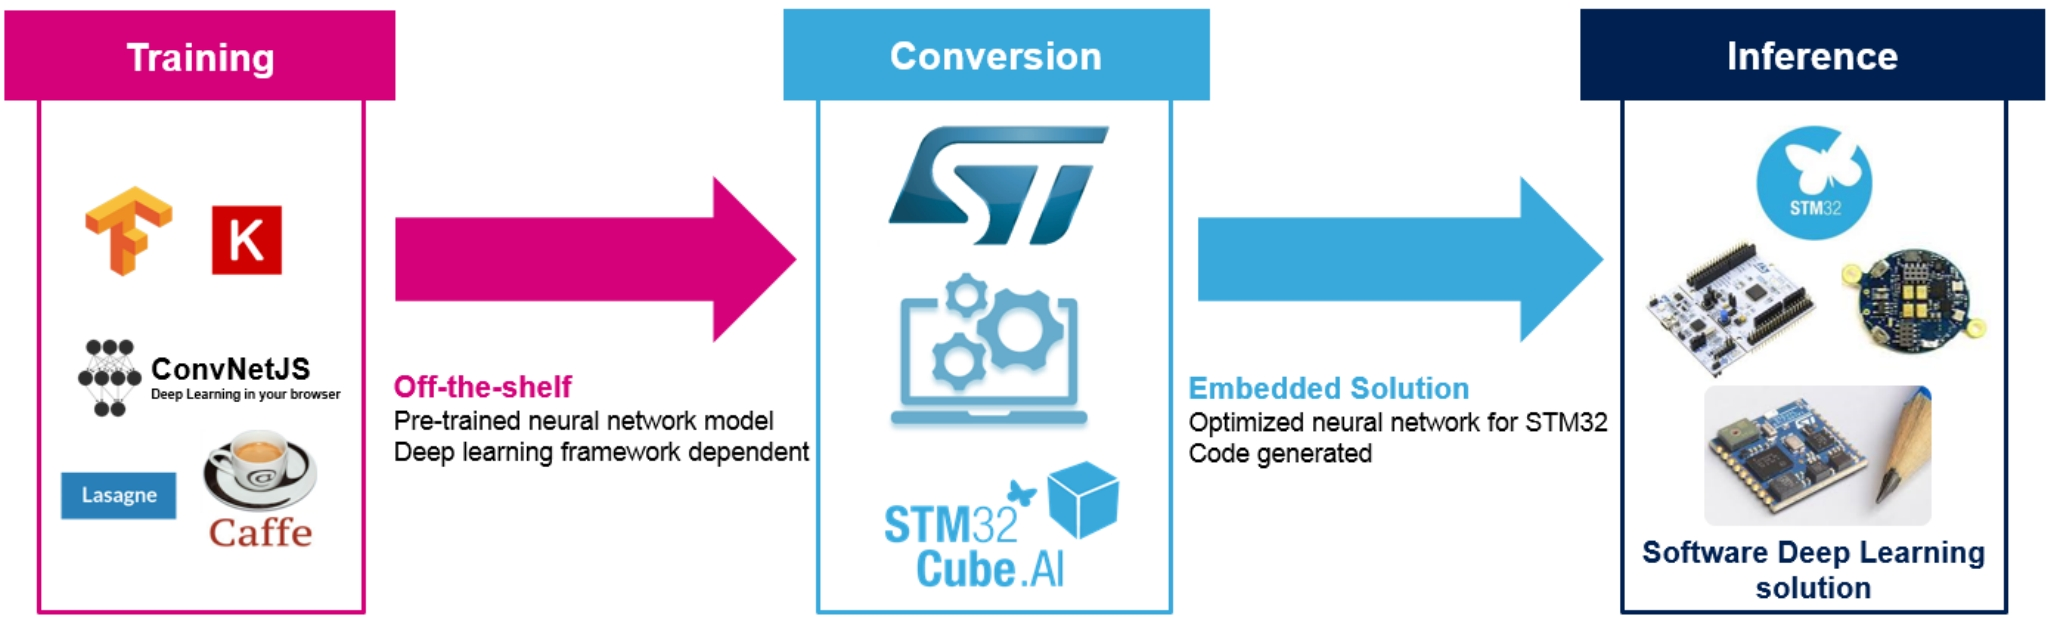
\includegraphics[width=.8\linewidth]{figures/content/chapter4/CUBEAI.jpeg}
  \caption{ X-CUBE-AI 概述}
  \label{fig:4_6}
\end{figure}


本文实验最终将优化后的神经网络模型部署于 Adhoc Deck 扩展板硬件平台上。
该扩展版以 STM32H743VIH6 微控制器为核心，辅以外部Flash存储器与FRAM非易失性存储器，形成了一套兼顾计算性能、存储容量与数据可靠性的嵌入式系统。
STM32H743VIH6 基于ARM Cortex-M7内核，主频最高可达480 MHz，具备较强的浮点运算能力和丰富的片上外设资源，可满足复杂算法在嵌入式环境下的实时运行需求。

在存储设计方面，系统采用多层次存储架构。
首先，微控制器内部集成2MB片上Flash存储空间。该存储器采用双存储块结构，每个存储块容量为1MB，并进一步划分为多个扇区。这部分存储空间用于存储系统核心程序与基础配置，并通过逻辑划分实现不同功能区域的隔离，包括Bootloader区、主固件区、配置区以及用户数据区。其中，Bootloader负责系统启动及固件更新管理，主固件区用于存储应用程序，配置区用于保存系统参数，而用户数据区则支持运行过程中的数据存储。

在存储体系设计方面，系统采用分层化的多级存储架构。首先，微控制器内部集成 2MB 片上 Flash 存储空间。该存储器采用双存储体（Dual-Bank）结构，每个存储体容量为 1MB，并进一步划分为多个扇区（Sector）。基于该片上 Flash，系统实现了功能分区，包括 Bootloader 区、主固件区、配置区以及用户数据区。其中，Bootloader 区用于系统启动与固件升级管理，主固件区用于存储应用程序，配置区用于保存系统参数，而用户数据区则用于支持运行过程中的数据存储需求。此外，系统预留独立的 Flash 扇区作为临时存储区，在固件升级过程中用于缓存新版本固件，从而实现安全可靠的在线升级机制。

为进一步提升系统的数据存储能力，Adhoc Deck 扩展板引入了外部 Flash（W25Q64），用于存储大容量数据，如运行日志、轨迹信息以及扩展资源文件。同时，系统集成了 FRAM（FM25CL64）作为高可靠性存储单元。相比传统 Flash 存储器，FRAM 具有更高的写入速度和极高的擦写寿命，且无需擦除即可直接写入，因而特别适用于频繁更新的关键数据（如系统状态与控制参数）的存储场景。

综上，Adhoc Deck 扩展板通过片上 Flash、外部 Flash 与 FRAM 的协同设计，在存储容量、访问效率及数据可靠性之间实现了有效平衡。其中，片上 Flash 保障系统运行与升级过程的安全性，外部 Flash 提供大容量数据支持，而 FRAM 则满足高频写入与关键数据保护需求。该多层次存储架构为后续算法的稳定运行与数据处理提供了坚实的硬件基础。

\begin{figure}[htbp]
    \centering
    \subfloat[正面]{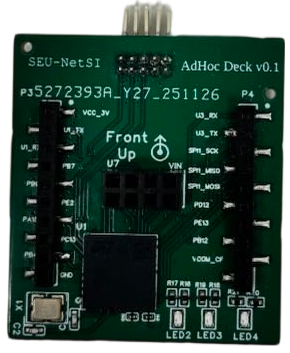
\includegraphics[width=.4\textwidth]{figures/content/chapter4/Adhoc正面.png}}
    \quad
    \subfloat[反面]{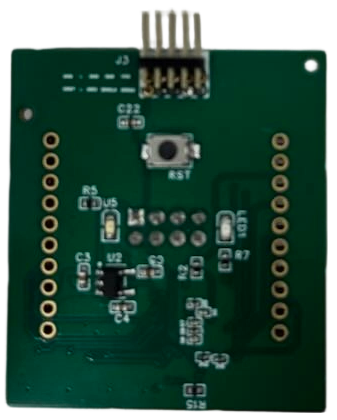
\includegraphics[width=.4\textwidth]{figures/content/chapter4/Adhoc反面.png}}
    \caption{部署平台：Adhoc Deck}
    \label{fig:4_7}
    \end{figure}

\subsection{网络模型的量化与部署}

在完成分布式强化学习模型的训练后，为实现其在嵌入式平台上的高效部署，需要将原始基于PyTorch框架的模型转换为硬件可执行的中间表示格式。为此，本文采用 ONNX（Open Neural Network Exchange）作为模型转换的中间桥梁，以实现模型从训练环境向嵌入式推理引擎的平滑迁移。

具体而言，首先对原始的 IQN模型进行结构封装，构建适用于导出的推理模型。在不改变原始网络结构与参数的前提下，对模型的前向传播过程进行显式展开，使其计算图能够被ONNX正确解析与表达。在该封装过程中，重点保留并规范化如下关键计算流程：状态特征提取、分位数特征映射、状态与分位数特征融合，以及分布式Q值估计。其中，分位数嵌入模块采用余弦基函数对采样分位点进行映射，并通过全连接层投影至高维特征空间，从而有效刻画动作价值的分布特性，增强模型对不确定性的表达能力。

为验证模型转换过程的正确性与稳定性，本文在Python环境下对转换前后的模型输出进行一致性检验。具体方法为：构造相同输入，分别输入至 PyTorch 模型与 ONNX 模型中，并计算两者输出 Q 值之间的最大绝对误差。实验结果表明，转换前后模型输出的最大误差控制在 $10^{-5}$ 以内，表明模型在转换过程中未引入显著数值偏差，具备良好的数值一致性，为后续嵌入式平台部署提供了可靠保障。图\ref{fig:4_8}展示了压缩后模型的网络图。
 \begin{figure}[htbp]
  \centering
  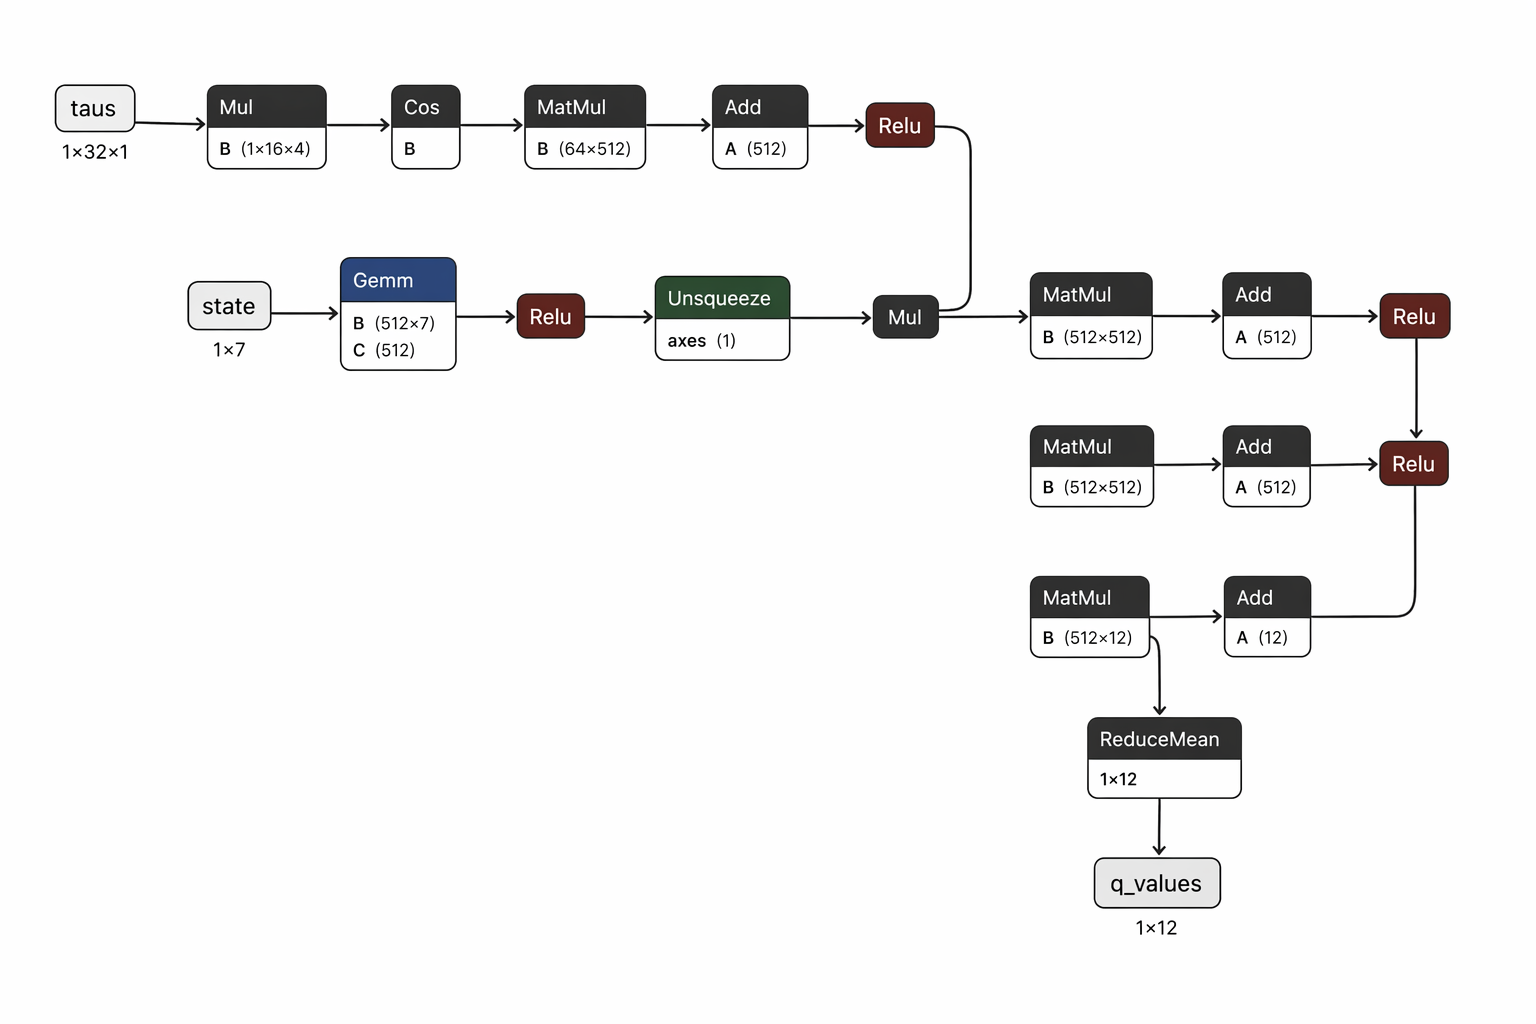
\includegraphics[width=.7\linewidth]{figures/content/chapter4/iqn_native.png}
  \caption{转换后的网络模型图}
  \label{fig:4_8}
\end{figure}

本文基于 STM32Cube.AI 提供的模型转换与部署工具链，对训练完成的模型进行了多层次优化处理。
整体而言，该优化过程并非单一压缩策略，而是由计算图优化、算子融合、权重量化、权重压缩、内存复用以及推理内核优化等多种技术协同构成。
首先，在模型转换阶段，通过对计算图进行静态分析，执行常量折叠与冗余节点消除等操作，将训练阶段中可预计算的部分提前固化，从而减少运行时计算负担；
同时，通过算子融合技术，将卷积层与批归一化层、激活函数等进行等效合并，在不改变模型表达能力的前提下减少中间张量的生成与存储开销，提高执行效率。
在此基础上，引入量化机制，将原始的 32 位浮点参数映射为低比特定点表示，显著降低模型参数存储规模，并使推理过程能够利用嵌入式处理器中的定点运算单元，从而在保证精度可控的前提下提升计算效率。

在上述优化手段中，权重压缩是降低模型 ROM 占用的关键技术之一，其具体实现过程如图\ref{fig:4_9}所示。原始网络模型中，各层权重与偏置参数（如 W1.conv、W2.dense、W3.dense）通常以 float32 形式分散存储，其总体大小由参数数量与数据精度共同决定，对应图中的未压缩存储结构（Un-compressed ROM size）。针对这一问题，CUBE-AI 首先对各层参数进行结构化重排，将不同层的权重与偏置按照统一顺序拼接为连续的内存块（memory chunk），从而提升数据访问的局部性，并为后续压缩提供统一的数据组织形式。在此基础上，结合量化后的低比特表示，对权重数据进行进一步压缩编码，将原始高精度参数映射为紧凑的定点表示，并通过统一格式进行集中存储。由图中“W′ compressed layer”可以看出，压缩后的权重不再与原始层一一对应，而是以压缩块形式重新组织，其中标注的“×4”表示相应权重存储规模约缩减至原始的四分之一，而“×1”则表示该部分压缩收益较低，基本保持原始比例。该过程本质上通过减少冗余表示与优化存储结构，实现参数的高效编码。

\begin{figure}[htbp]
  \centering
  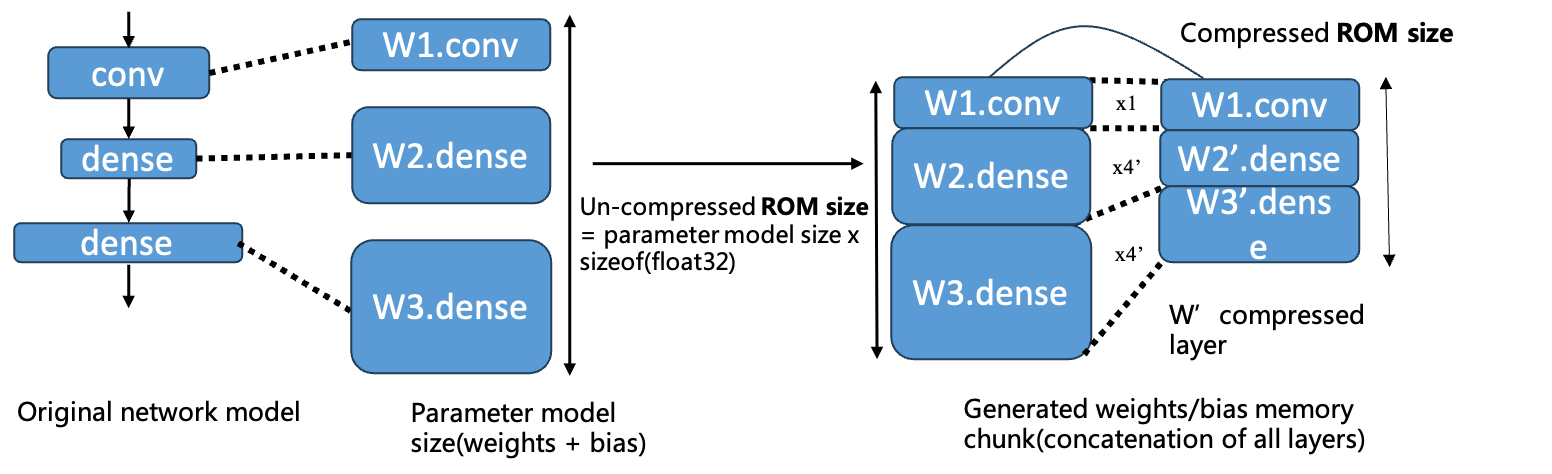
\includegraphics[width=.8\linewidth]{figures/content/chapter4/compressTheory.png}
  \caption{CUBE-AI权重压缩}
  \label{fig:4_9}
\end{figure}

在推理执行阶段，压缩后的权重通常以连续数组形式存储于 Flash 中，并在计算过程中按需读取，直接以定点形式参与运算或通过轻量级解码恢复必要精度，从而避免频繁的浮点转换操作，在保证计算正确性的同时兼顾存储效率与执行效率。通过上述机制，模型参数存储规模通常可降低至原始 float32 表示的约 1/4 甚至更低，显著缓解嵌入式平台的存储压力。此外，为进一步降低运行时内存占用，CUBE-AI 通过生命周期分析对中间张量进行内存复用，将不同计算阶段的缓冲区映射至同一物理地址，从而减少 RAM 使用量；同时采用静态内存分配策略，在编译阶段确定所有张量的内存布局，避免动态分配带来的额外开销与内存碎片问题。在推理执行层面，通过调用针对 ARM Cortex-M 架构优化的高效计算内核（如基于 SIMD 与 DSP 指令的实现），进一步提升模型运行速度。综上所述，该模型压缩与优化过程从存储表示、计算结构及执行机制多个层面协同作用，在保证模型精度基本稳定的前提下，大幅降低了模型对嵌入式硬件资源的需求，为复杂深度学习模型在资源受限环境中的高效部署提供了有效支撑。

如图\ref{fig:4_10}所示，给出了经仿真验证后的训练模型在压缩优化后的复杂度分析结果。
基于 STM32Cube.AI 生成的报告可知，模型单次推理的乘加运算次数（MACC）为18\allowbreak,033\allowbreak,384次，其中计算开销主要集中在中间的矩阵乘法层，单层占比约为 46.5\%，而激活函数及加法等操作的计算占比较低。
存储方面，模型在 Flash（ROM）中的占用为 572,636 Byte（约 559.21 KiB），全部由权重参数构成，表明量化与权重压缩已有效降低存储规模。运行内存方面，推理过程占用 RAM 为 34,816 Byte（约 34.00 KiB），主要用于中间激活值存储，输入输出占用极小且已包含其中。总体来看，压缩后的模型在计算复杂度、存储占用及内存使用之间实现了良好平衡，能够满足嵌入式平台的部署需求。

\begin{figure}[htbp]
  \centering
  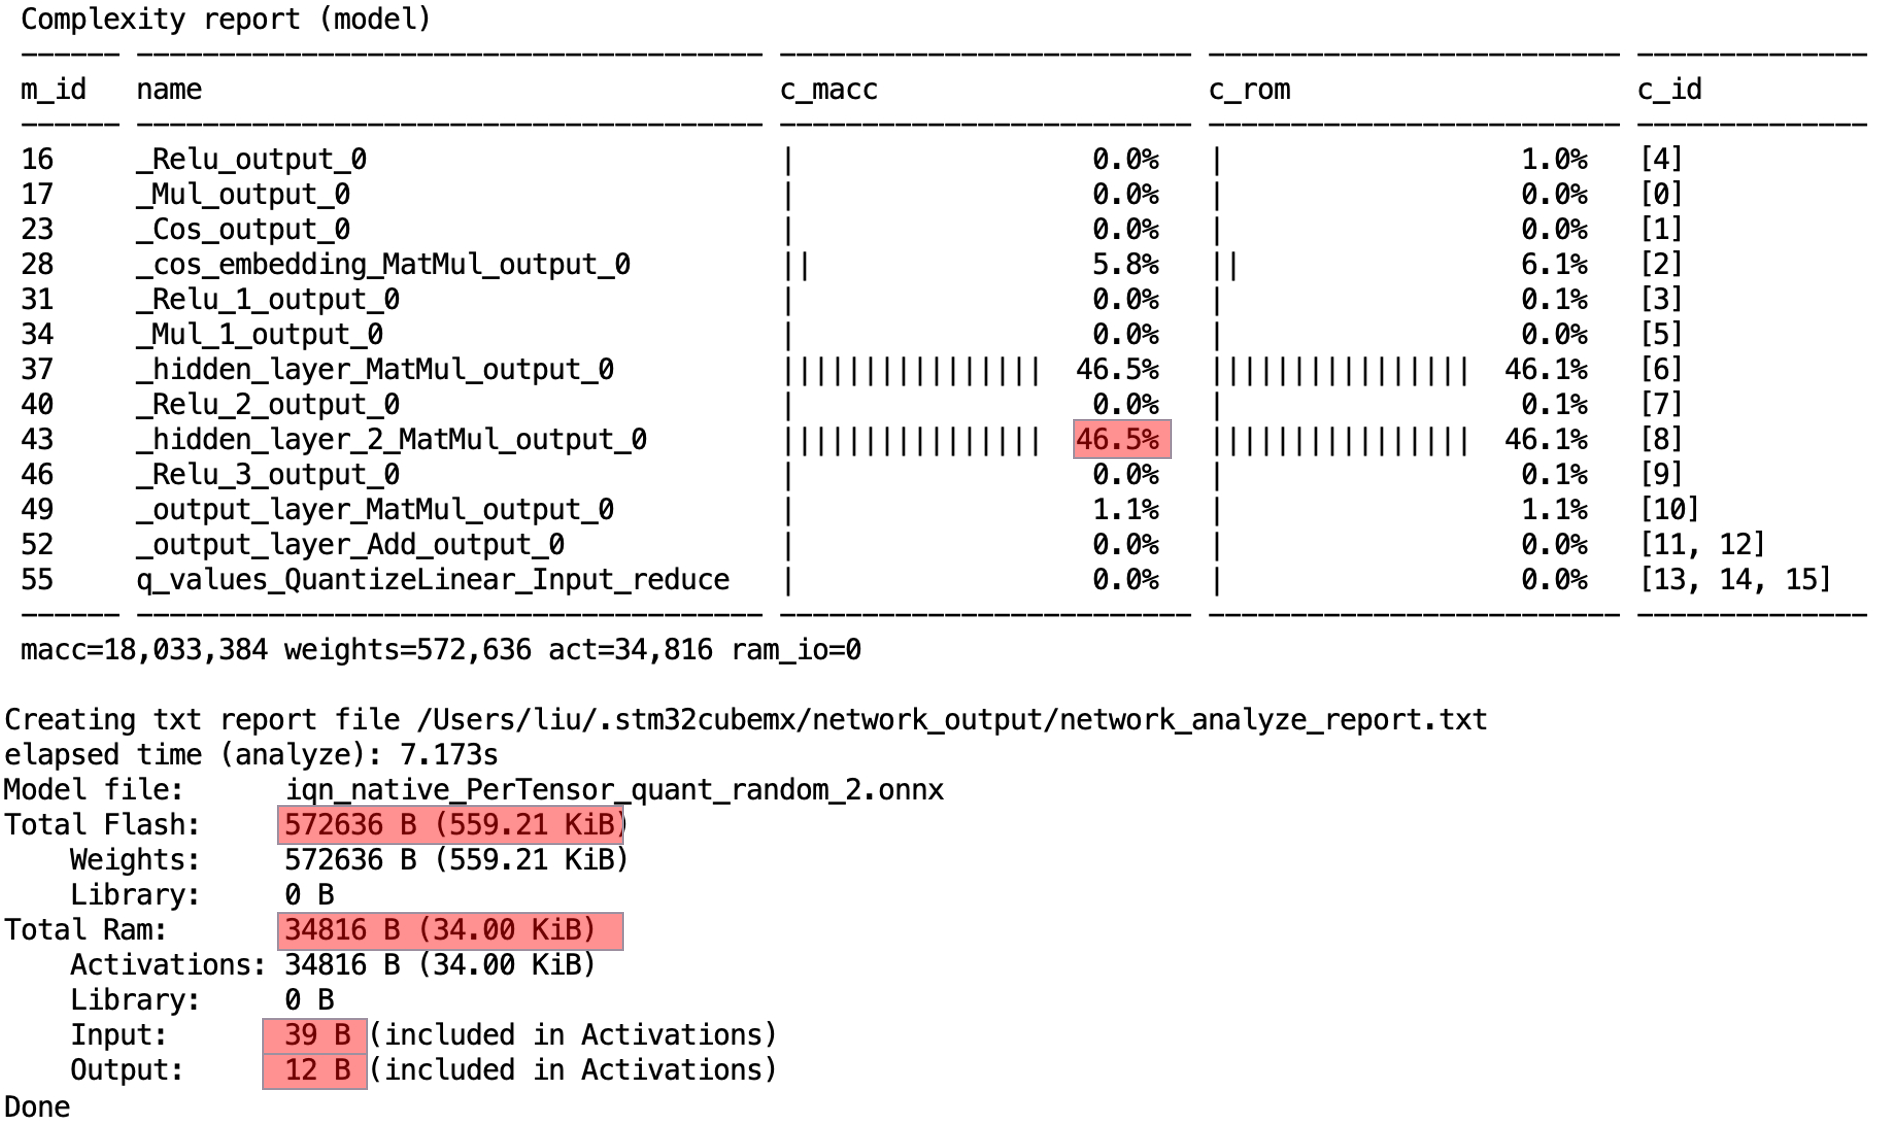
\includegraphics[width=.8\linewidth]{figures/content/chapter4/AIcompression.png}
  \caption{模型压缩结果}
  \label{fig:4_10}
\end{figure}
针对压缩后的模型，其具体的嵌入式部署方法如图\ref{fig:4_11}所示。
系统以 Adhoc Deck 扩展板为核心计算单元，用于分别存储运行时数据与压缩后的神经网络模型参数。
在该硬件平台上部署经优化后的IQN模型，实现飞行过程中的实时决策推理。

在模型部署流程中，首先将训练并压缩后的模型烧录至 Flash 存储器中，系统运行时由主控处理器加载相关参数并执行推理计算。模型以无人机当前状态信息作为输入，输出对应的动作价值估计或控制指令，从而实现对飞行行为的实时决策控制。整个推理过程在嵌入式端本地完成，无需依赖外部计算资源，从而保证系统的实时性与自主性。
在感知与通信方面，系统通过 Multi-ranger Deck 获取周围障碍物的距离信息，该模块通过I2C接口与无人机进行数据交互，实现环境感知输入的实时更新。
同时，外部定位系统采用 Vicon 动作捕捉系统，通过计算机端处理后生成高精度位姿数据，并经由 2.4G Crazyradio PA 无线通信模块发送至无人机，实现定位信息的闭环反馈。
嵌入式系统通过 UART 接口实现Adhoc Deck与无人机进行数据交互，实现模型输入输出与飞控控制指令之间的传递。
从整体数据流来看，系统形成了“环境感知—状态获取—模型推理—控制输出”的闭环结构：一方面，多源传感器（如测距模块与定位系统）提供实时环境与位置信息；另一方面，嵌入式端部署的 IQN 模型对输入状态进行推理，输出控制策略，并通过通信接口反馈至无人机执行机构，从而实现自主决策与避障控制。

综上所述，该部署方案充分结合了嵌入式计算平台与外部感知系统的优势，通过在资源受限的硬件环境中实现强化学习模型的高效推理，构建了一个具备实时性与自主性的无人机智能控制系统，为后续复杂环境下的自主导航与决策提供了可靠基础。
\begin{figure}[htbp]
  \centering
  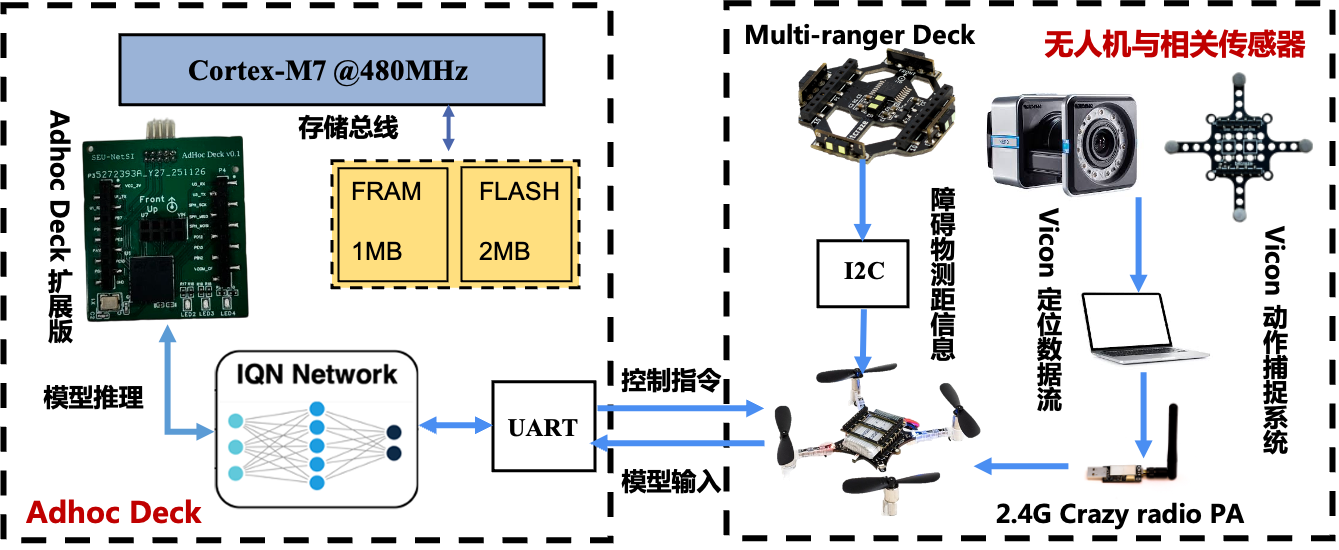
\includegraphics[width=.8\linewidth]{figures/content/chapter4/Adhoc与无人机交互.png}
  \caption{Adhoc Deck与无人机及其相关传感器交互}
  \label{fig:4_11}
\end{figure}

\subsection{真机实验结果分析}
本节基于上述算法与系统设计开展真机实验，以验证所提出强化学习导航算法在实际系统中的可行性与实时性。
首先对无人机硬件平台及其相关配置进行介绍，如图\ref{fig:4_12}所示，实验平台基于开源微型四旋翼无人机Crazyflie 2.1，并结合扩展计算模块Adhoc Deck构建边缘推理系统，实现模型在嵌入式端的在线决策能力与无人机导航功能。具体配置如下

\begin{figure}[htbp]
  \centering
  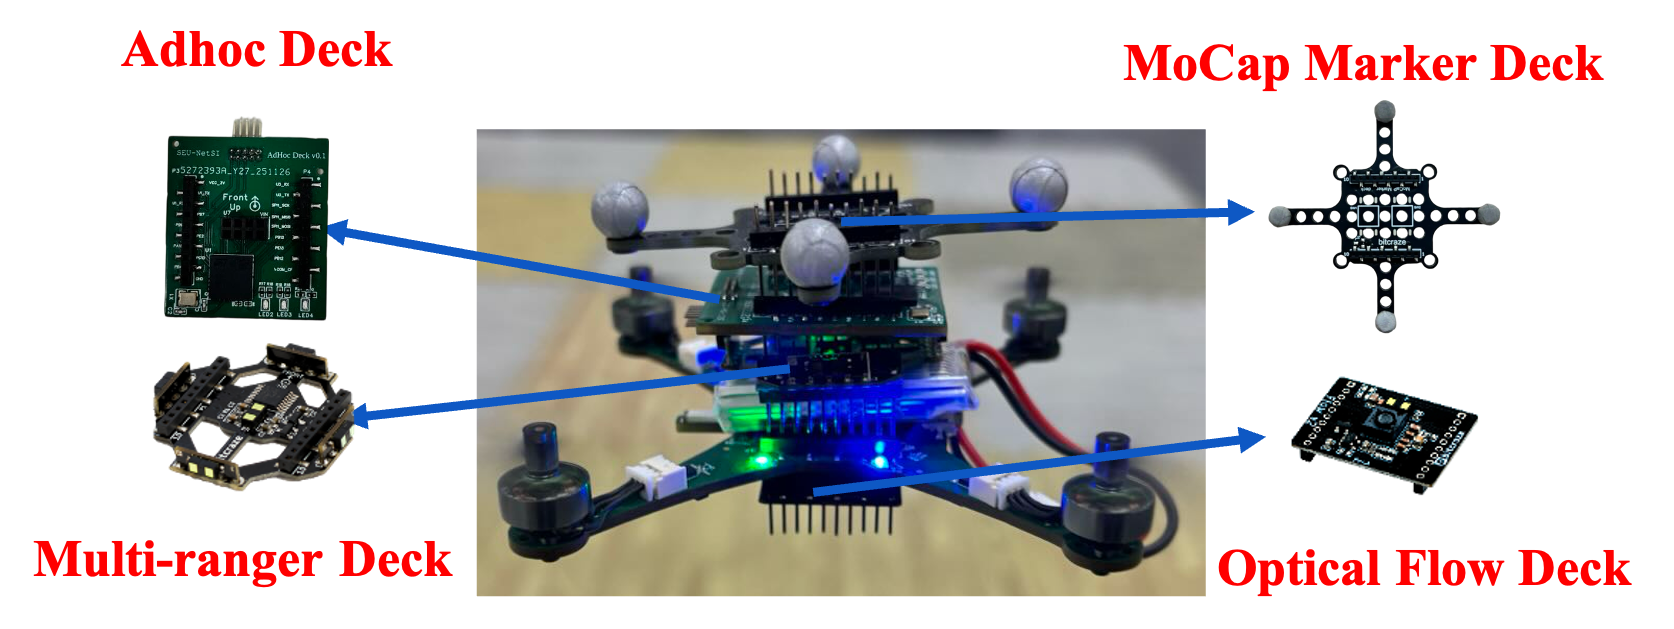
\includegraphics[width=.8\linewidth]{figures/content/chapter4/导航无人机.png}
  \caption{部署模型所用到的无人机及其扩展版}
  \label{fig:4_12}
\end{figure}

\begin{itemize}

  \item 嵌入式计算模块（Adhoc Deck）：作为模型推理的核心单元，搭载 Cortex-M7 处理器，负责执行压缩后的 IQN模型，实现实时路径决策与控制输出。
  
  \item 测距感知模块（Multi-ranger Deck）：由多个基于 ToF（Time-of-Flight）的激光测距传感器（VL53L1x）构成，分别安装于无人机前、后、左、右及上方方向，用于获取周围障碍物的距离信息，最终将数据传输至 Adhoc Deck，作为模型输入的一部分。
  
  \item 光流传感器模块（Optical Flow Deck）：由 VL53L1x 激光高度传感器和 PMW3901 光流传感器组成，可提供最高 100 Hz 的速度测量数据。
  
  \item 被动反光标记模块（MoCap Marker Deck）：由多个反光球组成，通过反射外部红外光源实现目标检测与识别，并由运动捕捉系统获取无人机的高精度位姿信息。
  
  \end{itemize}

  无人机真机导航任务在4.8×4.8米复杂环境中实施。如图\ref{fig:4_13}所示，在泡沫板场地中，我们在不同位置放置了形状大小各异的立方体作为我障碍物，并保证至少有一个障碍物在起点和终点的连线上，避免简单的直线飞行。

\begin{figure}[htbp]
  \centering
  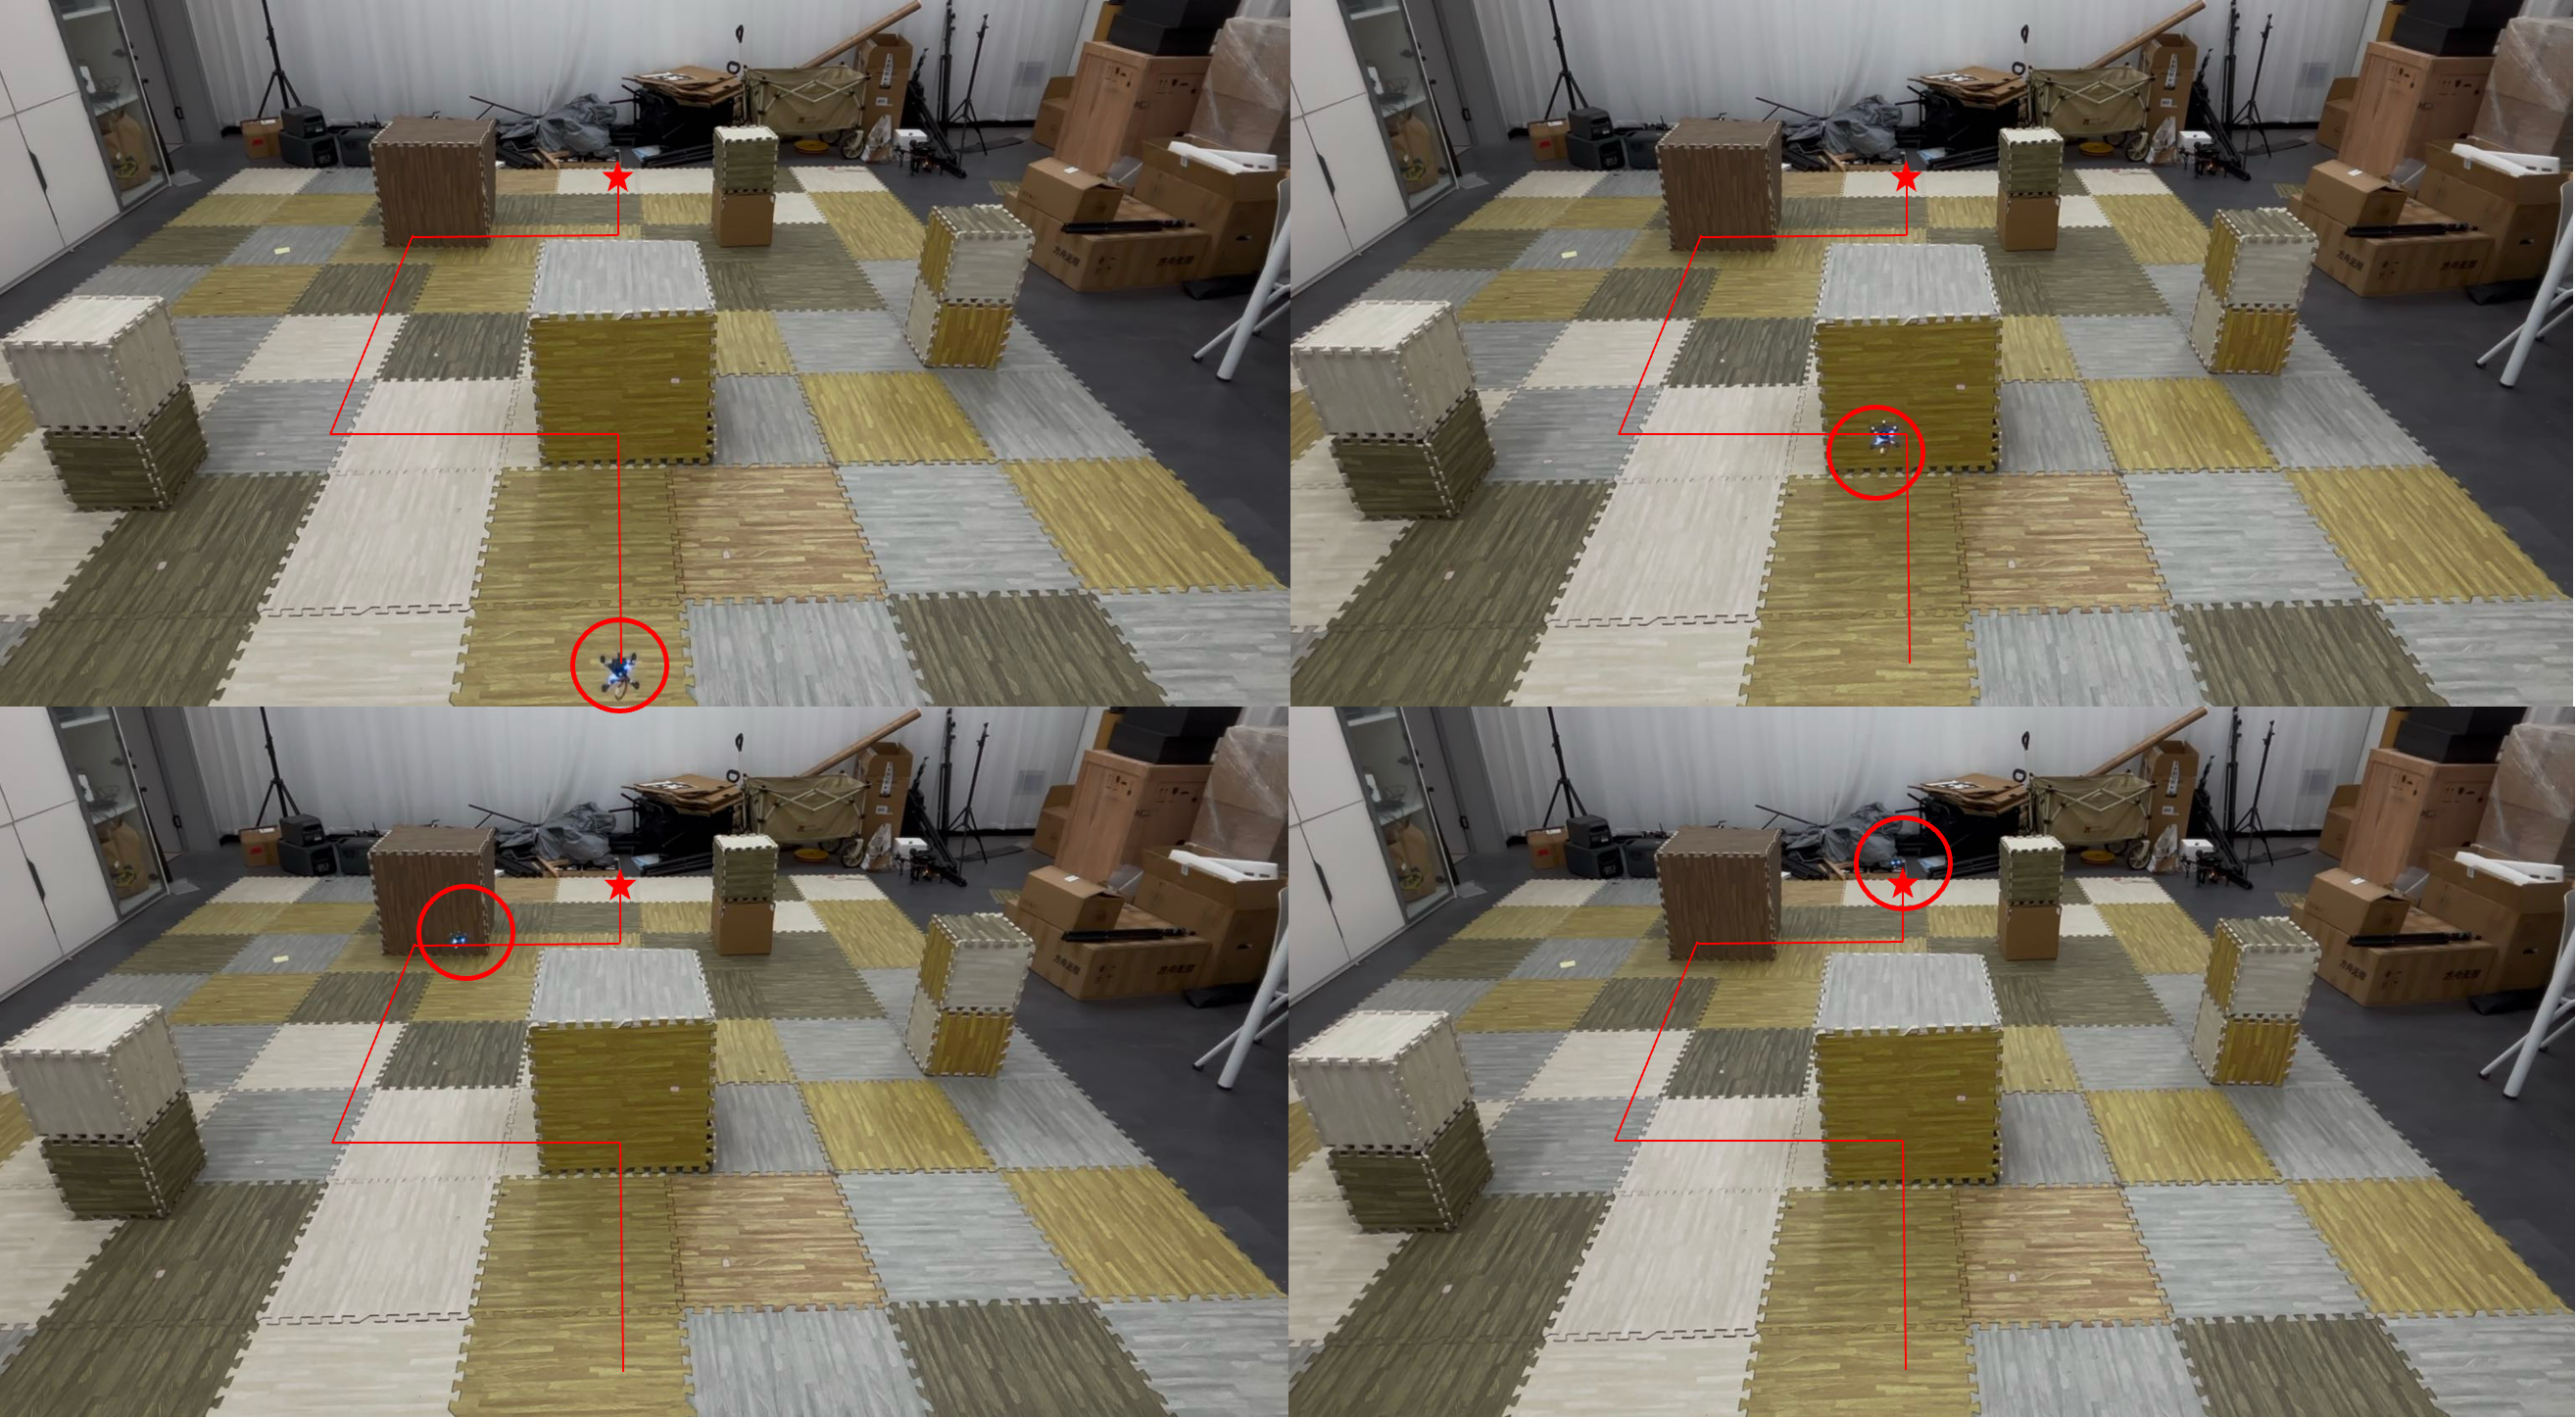
\includegraphics[width=.8\linewidth]{figures/content/chapter4/真机实验图.png}
    \caption{无人机自主导航实验图}
    \label{fig:4_13}
    \end{figure}

实验过程中，无人机需在未知环境中完成从起点到目标点的自主导航任务。
图\ref{fig:4_13}展示了实验过程中四个典型时刻的实拍图像，分别对应时刻1、时刻2、时刻3及时刻4。
在时刻2（图\ref{fig:4_13}(b)），无人机飞行至环境中第一个关键转折区域。面对局部障碍物或通道变化，导航系统实时更新路径规划策略，成功引导无人机调整航向，避免与周围环境发生碰撞。
最后，在时刻4（图\ref{fig:4_13}(d)），无人机成功抵达目标区域附近。此时，无人机已顺利完成导航任务，飞行轨迹收敛至目标点，整体导航过程平稳可靠。实验结果表明，本文方法能够在实际飞行条件下实现稳定、有效的自主导航。
\section{本章小结}

本章围绕无人机在复杂未知环境中的自主导航问题，系统地开展了从算法设计、模型训练到嵌入式部署与真机验证的完整研究工作。

首先，针对传统强化学习方法仅关注期望回报、难以应对低概率高风险事件的问题，本文在分布式强化学习框架下，引入回报分布建模思想，构建了基于隐式分位数网络的导航模型。在此基础上，提出了自适应风险倾向隐式分位网络算法，通过结合条件风险价值与回报分布特性，使智能体能够在决策过程中综合考虑收益与风险，从而提升在复杂环境中的安全性与鲁棒性。同时，引入右截断方差刻画内在不确定性，并基于其变化动态调整风险倾向，实现策略在风险规避与效率之间的自适应平衡。最后通过构建二维仿真环境并引入域随机化与渐进式训练策略，有效提升了模型的泛化能力。实验结果表明，相较于传统DQN及固定风险偏好的IQN方法，ART-IQN在成功率、碰撞率与导航效率等指标上均表现出更优的综合性能，验证了所提方法在复杂环境中的有效性。

在模型部署方面，针对嵌入式平台资源受限与实时性要求高的特点，本文基于STM32Cube.AI工具链对训练模型进行了量化、压缩。优化后的模型成功部署于Adhoc Deck扩展板，实现了端侧实时推理，并与Crazyflie 2.1无人机飞控系统协同工作，构建了“感知—决策—控制”的闭环自主导航系统。

最后，通过真实飞行实验对所提出方法进行了验证。实验结果表明，经过压缩优化后的模型能够在嵌入式硬件上稳定运行，并在实际复杂环境中实现有效避障与自主导航，具备良好的实时性与环境适应能力。


